\listoffigures

\chapter{Úvod}
Svět se neustále vyvíjí a~moderní doba vyžaduje moderní řešení. Společně s~vývojem technologií se mění i~očekávání jejich uživatelů. Velké množství populace se snaží udržet zdravý životní styl a~to má za následek tvorbu množství různých elektronických zařízení a~k nim aplikací pro usnadnění životosprávy.
    
Účelem bakalářské práce je poskytnout uživatelům fitness aplikací nový způsob motivace ke sportu a~to ve formě webové aplikace. Motivace je ve formě minihry, kde uživatel prochází světem a~aplikace mu následně přiřadí pomocí tzv. Voroného diagramu území, které zabral svoji trasou. Další funkcí aplikace je vytvoření průměrné trasy z~velkého množství tras, které vedly podobnou polohou. Toto se hodí v~případě, kdy má uživatel zájem aproximovat skutečnou trasu, kterou pravidelně prochází za pomocí průměrování jeho nasbíraných dat.
    
Druhá kapitola obsahuje rozvedené informace o~současných moderních aplikacích pro fitness. Zde jsou popsány způsoby, jakými získávají koncept GPS a~základní teorie o~databázi \emph{OpenStreetMap}. V~dalších sekcích jsou popsané různé funkce a~vlastnosti, které uživatelům poskytují současné fitness aplikace na trhu. Mezi nimi bylo nutné rozhodnout, které budou využity jako hlavní zdroj uživatelských dat pro bakalářskou práci. Zde jsou zváženy i~například zveřejněné průzkumy na webových stránkách od jiných uživatelů. V~poslední části je popsán samotný koncept Voroného diagramu, který je využit v~pozdější fázi implementace.
    
V následující kapitole je rozebrána tématika vytváření webových aplikací. Zde jsou analyzovány akce, které by aplikace měla uživateli zprostředkovat ve formě modelu případu užití. V~sekci~\ref{frameworks} jsou rozebrány moderní technologie, ze kterých si v~dnešní době vývojáři vybírají a~jejich případné výhody či nevýhody. Tato sekce je dále rozdělena dle typu informací na serverové a~klientské části. V~následující sekci jsou popsané druhy databází, které by mohly vyhovovat potřebám aplikace. V~předposlední části jsou zváženy různé knihovny, které poskytují zobrazení geografických map a~v jakých formátech pracují. Kapitola je ukončena návrhem samotného uživatelského grafického rozhraní.

Kapitola~\ref{implement} detailně popisuje použité technologie, algoritmy, vytvořené skripty a~náhledy do zdrojových kódu. V~rámci bakalářské práce je v~první sekci znázorněný postup pro vytvoření vlastní instance serveru pro zprostředkování vyhledávání mezi jednotlivými Voroného regiony.  Dále je zde popsané, jakým způsobem je možné vyextrahované data vložit do již existující databáze. V~sekci~\ref{userAppStravaConnection} je probírané téma implementace navázání spojení a~přístupů k~uživatelským datům, následně je řešena otázka škálování při zpracování dat. Samotná sekce zpracování v~sobě obsahuje velké množství implementačních detailů a~problémy, které byly řešeny v~době vývoje serverové části. V~poslední řadě jsou obdobně vysvětleny detaily a~různé funkce, které byly implementovány pro uživatelský komfort v~klientské části. 

V předposlední kapitole je znázorněno testování různých uživatelských funkcí zmíněných v~modelu případu užití. Aplikace procházela intenzivním testováním již během samotného vývoje, kdy bylo nutné neustále kompilovat zdrojové kódy pro ověření funkčnosti. Zde popsané testy mají ve většině případů reference na přílohu~\ref{test:app}, která obsahuje vytvořené obrázky jako výstup testování. 

Na konci práce je přidáno několik příloh, které usnadní zájemcům, kteří by chtěli aplikaci otestovat práci. V~příloze~\ref{startapp} se vyskytuje manuál ke spuštění, kde jsou popsané nutné prerekvizity a~příkazy pro kompilaci aplikace. Příloha~\ref{sqlserverpictures} zobrazuje možné vložení souboru dat do databáze pomocí \emph{Microsoft SQL Server Management Studia}.

\chapter{Problematika OpenStreetMap, GPS a~Voroného regionů}
\label{theory}
V kapitole je popsána teoretická stránka geografických informací a~jejich získání, které tvoří základ dat, které aplikace požaduje.

\section{OpenStreetMap}
OpenStreetMap je projekt zabývající se budováním volně dostupné geografické databáze světa. Jejím cílem je získat informační záznam o~každém geografickém rysu. Zpočátku se jednalo hlavně o~mapování cest a~silnic, delší dobu už ale obsahuje i~informace o~polních cestách, budovách, poštovních schránkách, vodních tocích, lesích, plážích atd. Pro potřeby dnešní doby také obsahuje data o~autobusových linkách, různých obchodech a~dalšími daty infrastruktury. Drtivá většina databáze je vytvořena díky spolupráci veřejnosti a~příspěvkům uživatelů OpenStreetMap. \cite{openstreetmap}

Tyto data se sbírají například během provozování cyklistiky nebo i~chůzí po cestách a~v~přírodě. Pro záznam těchto dat je využita různá nositelná elektronika (angl. \emph{Fitness Trackers}). Ty se nejčastěji vyskytují ve formě chytrých hodinek a~náramků, které jsou spojeny s~mobilní nebo webovou aplikací. Většina nositelné elektroniky využívá tzv. \emph{globální polohový systém} neboli GPS ke~sběru dat. \cite{trackers}
\section{Globální polohový systém}
Na počátku stála myšlenka touhy po lehkém určení polohy při cestování. Principiálně GPS satelity vždy znají svoji vlastní polohu. Ke každému zařízení, které se ptá na jeho polohu jsou přiřazeny čtyři satelity. Tři jsou využity pro koncept resekce (angl. \emph{Navigation Resection})\footnote{Výpočet polohy pomocí resekce: \url{https://www.armystudyguide.com/content/army_board_study_guide_topics/land_navigation_map_reading/find-your-location-using-.shtml}}, pro výpočet polohy zařízení. Čtvrtý satelit zajišťuje správnou funkci časového čítače přijímacího zařízení. \cite{gps3} 

\subsubsection*{Historie}
V~prosinci 1973 byl schválen program GPS. Během následujících několika let bylo na orbit vysláno několik satelitů. V~roce~1993 počet satelitů dosáhl~24. Právě díky těmto satelitům je veřejnosti přístupná technologie globálního zjišťování polohy. \cite{gps1}

Od této doby se GPS stal nezbytnou součástí infrastruktury celosvětově. Je využíván v~letectví, námořnictví, pro armádní účely, ale~i~v běžném životě pro navigaci pěší nebo~v~autě za pomoci např.~mobilních a~webových aplikací. \cite{gps2}

V roce 1990 vláda USA zavedla selektivní dostupnost. Díky tomu byla přesnost pro GPS systémy pro civilní užití snížena na okolí 100 metrů. V~následujících letech si ovšem vláda uvědomila, jaké výhody má GPS i~pro civilní využití, v~roce 2000 byla selektivní dostupnost zrušena a~od té doby se přesnost rapidně zvýšila. \cite{gpsacc2}

V současné době většina nositelné elektroniky využívá přijímač na jedné GPS frekvenci. To poskytuje uživateli přesnost v~rozmezí 4.9~metrů pod širým nebem. Pro profesionální použití lze přesnost dále zvýšit za pomocí více GPS frekvencí, ale kvůli provozní ceně se dvě frekvence nedají využít pro příležitostné uživatele.  \cite{gpsacc1}

\subsection{Formát GPS}
Pro přenos a~uchování dat GPS se používá systém zeměpisných souřadnic (angl. \emph{Geographic Coordinate System}). Jednotlivé souřadnice jsou složeny ze zeměpisné šířky a~délky. Šířka je úhel mezi olovnicí v~daném bodě a~rovinou rovníku. Délka je úhel vzepětí mezi rovinou nultého poledníku a~rovinou poledníku daného bodu na zemském povrchu. Z~předchozí definice vyplývá, že samotný systém je ovlivněný tvarem Země.~\cite{gcs}

\section{Aplikace vyžívající GPS} 
\label{appcomparison}
\subsection{Endomondo}
\emph{Endomondo} byla aplikace od populární fitness firmy \emph{Under Armour}. Vyskytovala se výhradně jako mobilní aplikace, existovala placená i~neplacená verze. V~neplacené verzi se vyskytovaly reklamy, které mohli uživateli znepříjemnit její používání. Jedna z~oblíbených funkcí byla možnost malého odpočtu během aktivity. Poskytovala uživateli motivaci k~většímu výkonu po určitý časový interval, většinou v~rámci vteřin. Jednou z~nejvíce chválených funkcí bylo propojení s~dalšími uživateli, ti mohli v~reálném čase mezi sebou komunikovat a~to~i~během nahrávání aktivit. Aplikace měla možnost povzbuzujících hlášek, které si mohli uživatelé navzájem posílat i~během běhu. \cite{endomondo} 

K~záznamu pohybových dat aplikace využívala GPS polohu, kterou získala z~GPS zařízení v~mobilním telefonu uživatele. Pro zobrazení dat využívala \emph{Google Maps}. Po dokončení aktivity je bylo možné exportovat do \emph{.gpx} souborů, které jsou popsány v~sekci~\ref{gpx}. Podpora aplikace \emph{Endomondo} byla zrušena k~31.~prosinci 2020 a~byla nahrazena sesterskou aplikací \emph{MapMyRun}. \cite{endomondo}


\subsection{MapMyRun}
\emph{MapMyRun}\footnote{MapMyRun stránka: \url{https://www.mapmyrun.com/dashboard}.} byla vytvořena a~cílena na komunitu v~zahraničí, v~USA. Úsudek vychází z~přednastavených hodnot při prvním přihlášení a~následně implicitní pozice mapy.
Po vytvoření uživatelského účtu a~pokusu najít vytvořené cesty uživatelů v~okolí Brna vyšlo najevo, že v~České Republice tato aplikace nemá velké klientské zastoupení, doporučené trasy jiných uživatelů byly až deset let staré\,--\,z roku 2012.

Jak bývá mezi fitness aplikacemi obvyklé, pro záznam aktivit se využívá mobilní aplikace. Po zapnutí aplikace je viditelné \uv{Start} tlačítko, které zapne nahrávání tempa a~polohy. Aplikace umožňuje také spočítat spálené kalorie po dokončení aktivity nebo vytvoření šablony tréninkové trasy. Samozřejmostí je uživatelské přizpůsobení domovské stránky, lze nastavit metrický systém nebo třeba formát dnešního data. V~placené verzi aplikace poskytuje zvukovou zpětnou vazbu jako je čas, uběhlá vzdálenost a~tempo během aktivity. V~nástroji lze nastavit cíle, na které uživatele bude aplikace následně upozorňovat, pokud se k~nim atlet během aktivity přiblíží. \cite{stravavsmapmyrun,mapmyrun} 

\emph{MapMyRun} poskytuje oficiální API (angl. \emph{Application Programming Interface}) pro vývojáře, ovšem pro registrování vlastního API je nutno vyslovit zájem o~získání vlastního klíče a~poté existuje šance, že povolení bude uděleno. Společně s~malým množstvím českých uživatelů by bylo její využití nepraktické.
\subsection{Garmin}
\emph{Garmin} je firma, která se soustředí na fitness doplňky a~životní styl. Problematikou zobrazování uživatelských dat se zaobírá až webová aplikace nazvaná \emph{Garmin Connect}\footnote{Garmin Connect: \url{https://connect.garmin.com/modern/}.}. Stránka vypadá moderně, ale nemá žádné funkce, které by dále zpracovávaly údaje o~jednotlivých trasách. Poskytuje uživateli motivaci dále sportovat pomocí cílů, které si může nastavit. Vyskytuje se i~možnost sdílet aktivity s~přáteli v~reálném čase. 

Pro záznam polohy \emph{Garmin} využívá svoje vlastní zařízení, jedná se o~různé druhy nositelné elektroniky jako jsou hodinky a~náramky. Vyrábí i~samostatné zařízení GPS, které našly využití i~pro vojenské využití. Zařízení od \emph{Garmin} z~principu nevyužívají paměťové karty a~data o~aktivitě zaznamenává do své pevné paměti. Elektronika často obsahuje USB port pro připojení k~počítači, zde lze poté využít aplikaci \emph{Garmin Express} pro zobrazení nasbíraných dat.~\cite{garmin} 

\subsubsection{Garmin a~vývojáři}
Firma \emph{Garmin} vytvořila vlastní protokol FIT (angl. \emph{Flexible and Interoperable Data}\\\emph{Transfer})\footnote{FIT Protokol: \url{https://developer.garmin.com/fit/overview/}}. Pomocí tohoto protokolu lze sdílet data mezi různými platformami a~zařízeními. Využívá se pro záznam a~přenos nasbíraných fitness dat, např. mezi počítačem a~mobilem v~souborech formátu \emph{.FIT}.~\cite{garminfit} 

Garmin dále poskytuje přístup k~aktivitám uživatele pomocí tzv.~REST~API\footnote{Garmin REST API: \url{https://developer.garmin.com/gc-developer-program/activity-api/}.} (angl.
\emph{Representational State Transfer Application Programming Interface}). Pro přístup k~této technologii je ovšem nutné být registrovanou firmou a~teprve poté lze zažádat o~povolení. Pokud by aplikace měla být v~budoucnosti publikována širokému publiku, tak se Garmin dá považovat jako možné rozšíření. Ovšem v~rámci bakalářské práce je její využité obdobně jako aplikace \emph{MapMyRun} velice nepraktické.

\newpage
\subsection{Strava}
\label{strava}
Pokud člověk vyhledá na webu \uv{Fitness aplikace}, tak jedno z~nejvíce opakujících se jmen bude Strava. Strava je poskytnuta uživatelům ve formě webové, ale i~mobilní aplikace. Vyskytuje se zde možnost předplatného, kdy následně uživatel dostane přístup k~více funkcím a~statistikám. Uživatel zaznamenává data výhradně pomocí propojené mobilní aplikace. Před začátkem nahrávání aktivity se Strava zeptá na její typ, správný výběr aktivity následně umožňuje detailnější výpočet uživatelských statistik. Aktivity mohou být například ~běh, chůze, cyklistika, ale i~různé sporty. V~dalších sekcích aplikace je možné zúčastnit se \uv{Doporučených aktivit,}
což jsou trasy již zaznamenány a~doporučeny jinými uživateli. Samotný proces navrhnutí takovéto trasy se poté vyskytuje ve webové aplikaci. Uživatel má v~mobilní aplikaci také možnost znovu spuštění jeho již jednou provedených aktivit za účelem zlepšení času na trati. Pokud má uživatel zájem, může si přidat ostatní uživatelé jako přátelé a~následně společně vytvářet a~plnit různé fitness výzvy. 

Při nahrávání aktivity má uživatel v~aplikaci možnost výběru ze dvou druhů zvukových zpětných vazeb. V~neplacené verzi aplikace uživateli sděluje jeho současné tempo např. každého půl kilometru, toto chování se odvíjí dle nastavení. Dále zde existuje nástroj \emph{Live Segment Performance}, který uživateli dovolí si předem zvolit, ve kterém úseku by chtěl dostávat zvukové připomínky. Tento nástroj si pečlivý uživatel může nastavit jako pomocnou sílu v~obtížných úsecích, jako je např.~běh do strmého kopce.~\cite{stravavsmapmyrun}

Webová aplikace vypadá velice moderně a~poskytuje velké množství funkcí, které by průměrný uživatel očekával. Funkce jako zobrazení již existujících aktivit a~jejich správa, je samozřejmostí. Dále zde má uživatel možnost vytvářet vlastní trasy, jak bylo dříve zmíněno. Nástroj pro vytváření má dodatečné funkce na rozdíl od podobného nástroje v~\emph{MapMyRun}. Při práci s~nástrojem uživatel může povolit funkci doporučení tras. Následně uživateli Strava aktivně navrhuje další zajímavá místa, které jsou oblíbené a~doporučeny dalšími uživateli. Tyto populární ulice a~místa se také dají zobrazit pomocí jiného režimu mapy, tzv. \textbf{teplotní mapa}, (angl. \emph{Heatmap})\footnote{Heatmapa v~aplikaci Strava: \url{https://www.strava.com/heatmap}.}. Oddálenou mapu střední Evropy lze vidět v~obrázku~\ref{heatmap}. 
Pomocí zabarvení cest zobrazuje, jak často se uživatelé pohybují ve stejných místech, např. ulicích.
Aktivováním předplatného lze vidět data pro přihlášeného uživatele, v~neplacené verzi jsou to pouze obecná data všech uživatelů.~\cite{strava}

\subsubsection{Strava a~vývojáři}
Strava poskytuje oficiální a~veřejně dostupné API, které mohou vývojáři použít k~práci s~daty jednotlivých uživatelů\footnote{Strava, pro vývojáře: \url{https://developers.strava.com/}.}. Postup registrace vlastní aplikace je dále popsaný v~sekci~\ref{registerstrava}. Sekce~\ref{oauth} poskytuje podrobnější popis autorizace uživatelům. Z~důvodu zvýšení bezpečnosti citlivých uživatelských údajů Strava využívá protokol \emph{OAuth2} pro autorizaci jednotlivých uživatelů do aplikace třetí strany. Po schválení autorizace uživatelem získává aplikace přístup k~jeho aktivitám z~databáze Stravy. 
\begin{figure*}[h]
    \centering
    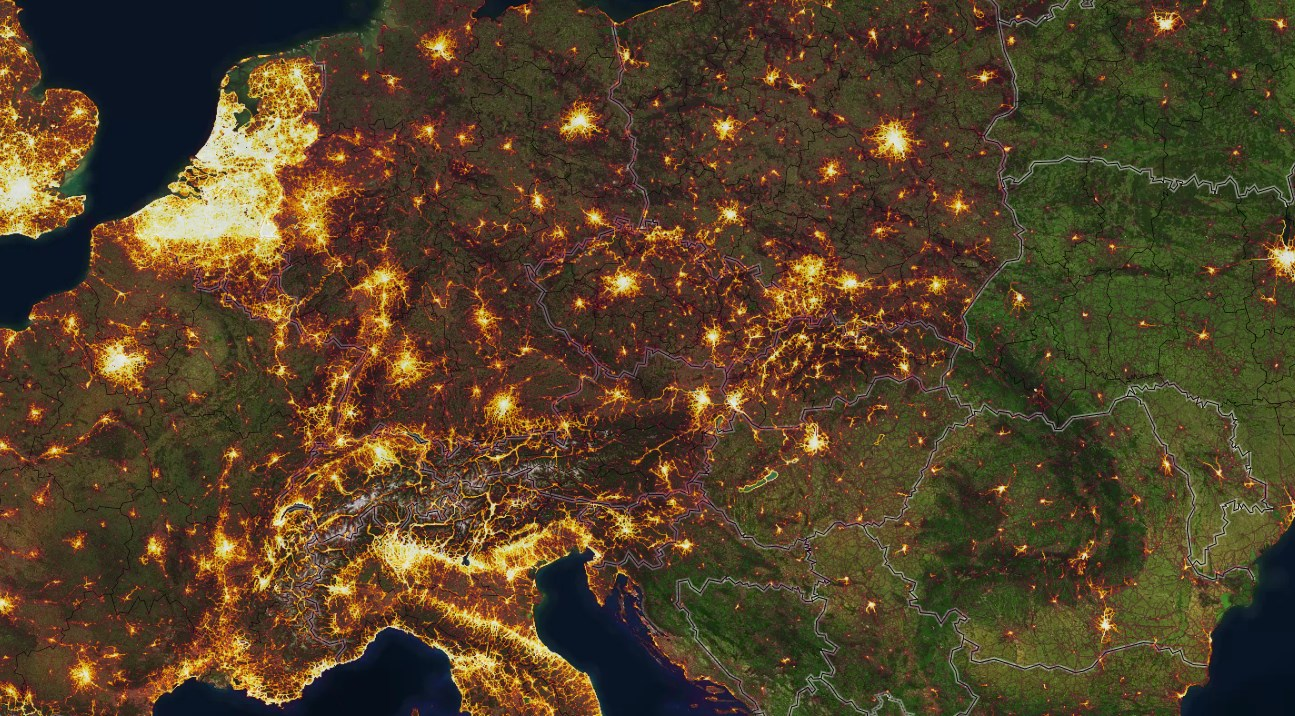
\includegraphics[width=0.94\textheight, angle=90]{obrazky/heatmap.jpg}\\[1pt]
    \caption{Heatmapa střední Evropy dle aplikace Strava}
    \label{heatmap}
\end{figure*}

\newpage
\clearpage
\section{Voroného diagram}
\label{voronoi}
Voroného diagram je rozdělení prostoru na základě množiny bodů $M$. Množina všech bodů prostoru, které jsou blíže k~prvku $a,\,a\in M$ než jakémukoliv jinému bodu z~množiny $M$ se nazývá Voroného region. V~obrázku~\ref{voronoi_streets} lze vidět zabrané území uživatelem s~modrou barvou trasy. Následně je jeho region vybarvený červenou barvou. Zelené a~červené tečky znázorňují středy Voroného regionů. Jednotlivé regiony byly vypočítány pomocí knihovny \emph{Scipy}.~\cite{voronoi} 

Pro využití Voroného regionů k~přiřazení území, které uživatel zabírá, bylo nutno připravit několik elementů:
\begin{itemize}
    \item Knihovna \emph{Scipy} a~její funkce \emph{Voronoi}. Tato funkce počítá hranice jednotlivých Voroného regionů. \cite{scipy}
    \item Množina $M$\,--\, databáze OSM (angl. \emph{OpenStreetMap}) obsahující informace o~cestách.
    \item Trasy uživatelů.
\end{itemize}
\vspace{1cm}
\begin{figure}[h]
    \centering
    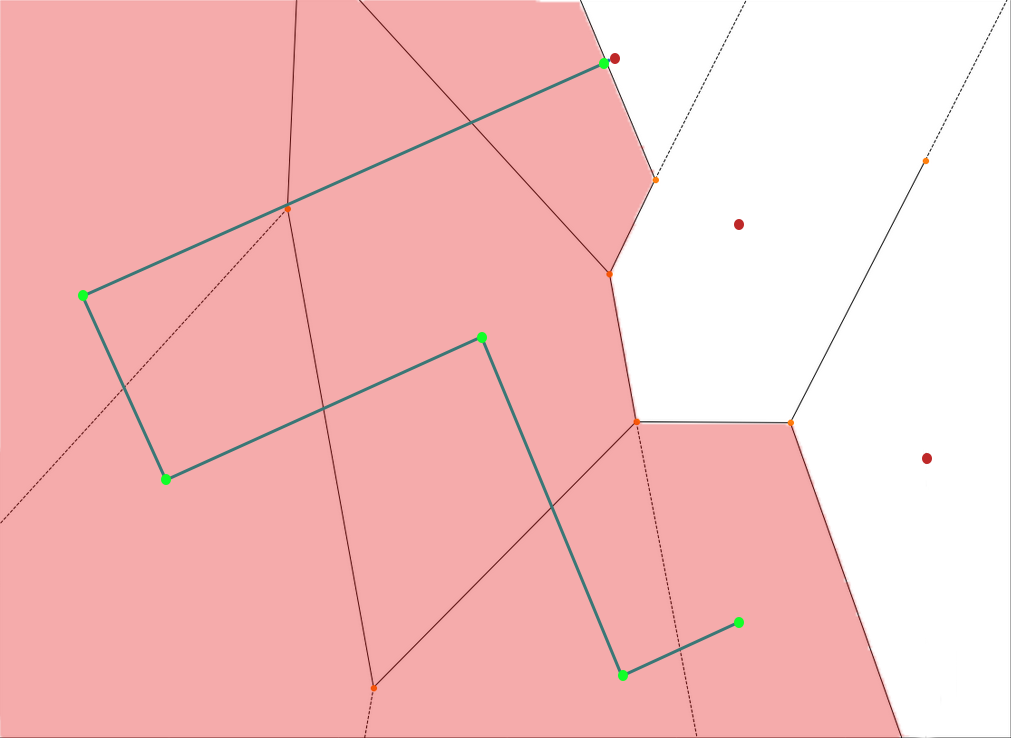
\includegraphics[width=0.85\textwidth]{obrazky/voronoiStreetsColored.png}
    \caption{Vyplnění regionů dle Voroného diagramů}
    \label{voronoi_streets}
\end{figure}
\newpage
Pro přehlednější ukázku funkce \emph{Voronoi} bylo využito prostředí \emph{Jupyter Notebook}\footnote{Jupyter Notebook dostupný z~\url{https://jupyter.org/}.}. Původní trasa byla ulice Bochořáková, která je viditelná v~obrázku~\ref{vor_regionsbase}. Výsledek výpočtu dle funkce lze vidět v~obrázku~\ref{vor_regions}, zde jsou středy regionů znázorněné modrou tečkou. 
\begin{figure}[h]
    \centering
    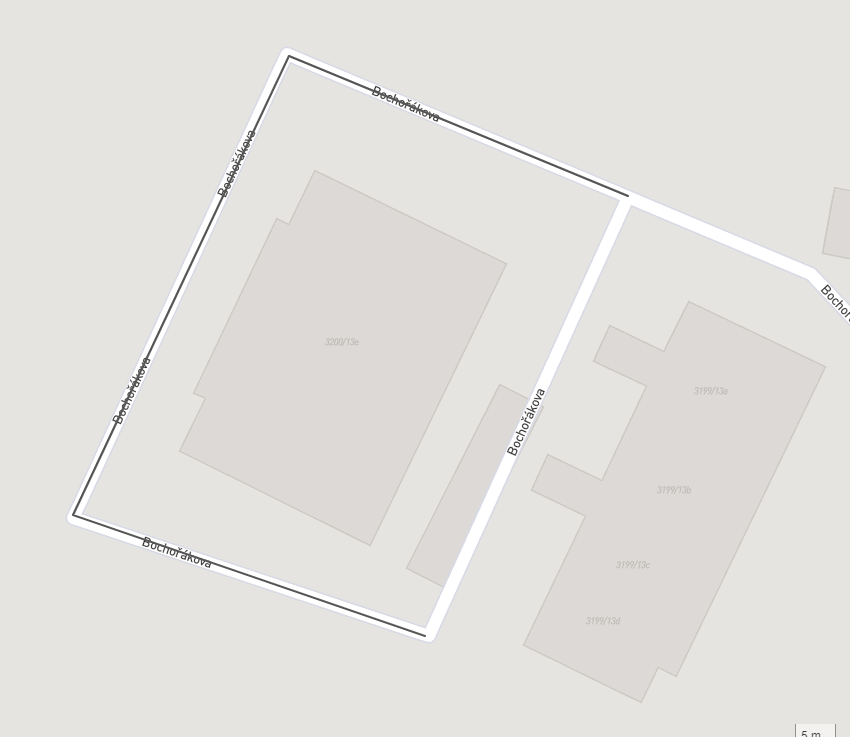
\includegraphics[width=0.55\textwidth]{obrazky/street.png}
    \caption{Ulice Bochořákova}
    \label{vor_regionsbase}
\end{figure}
\vspace{2cm}
\begin{figure}[h]
    \centering
    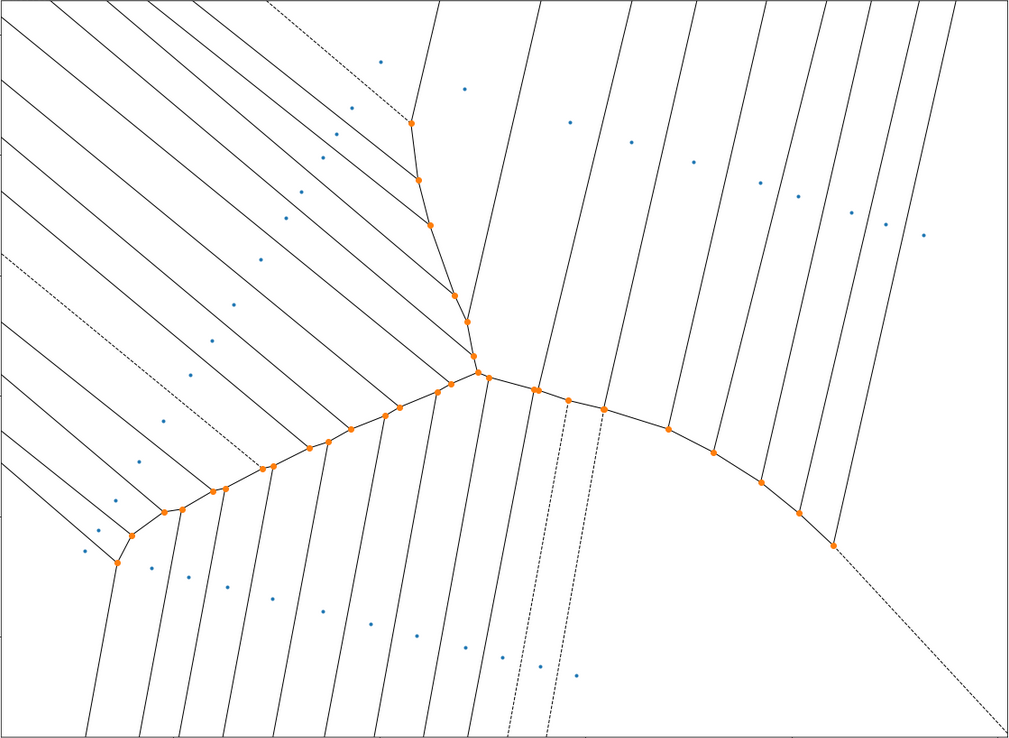
\includegraphics[width=0.7\textwidth]{obrazky/voronoi.png}
    \caption{Voroného regiony zobrazené pomocí Jupyter Notebook}
    \label{vor_regions}
\end{figure}

\chapter{Návrh webové aplikace}
\section{Analýza webové aplikace} 
Webová aplikace se bude nejvíce soustředit na zobrazení různých zpracovaných dat. Je tedy důležité, aby grafický design byl uživatelský příjemný a~poskytoval uživateli různé volitelné přizpůsobení. Je vhodné, aby si webovou stránku uživatel také mohl zobrazit z~mobilního telefonu, a~tedy je zde požadavek responzivity. Akce nutné implementovat pro uživatele dále popisuje model případů užití (obrázek~\ref{usecase}).
\subsubsection{Model případu užití}
\vspace{1.5cm}
\begin{figure}[h]
    \centering
    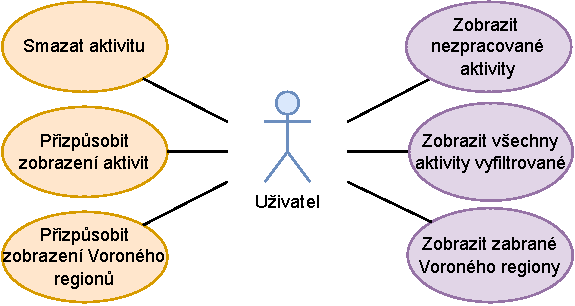
\includegraphics[width=0.85\textwidth]{obrazky/Use Case.pdf}
    \caption{Model případů užití}
    \label{usecase}
\end{figure}
\newpage
\section{Webové frameworky}
\label{frameworks}
Framework je obecně základní struktura pro systém. V~programování je framework nástroj, který poskytuje komponenty, objekty, nástroje a~nebo další programy, které jsou připravené pro použití vývojářem. Často jsou strukturovány do tzv. knihoven, jazyk ve kterém jsou napsané záleží hlavně na cílovém použití. Jejich cílem je usnadnit vývoj a~poskytnout standard pro programování na nízké úrovni, aby se vývojáři mohli soustředit na implementaci sekcí, které učiní jejich projekt výjimečným. Využití frameworku zvyšuje rychlost programování a~zjednodušuje testování. Frameworky aktivně vyvíjené jeho komunitou často mívají náskok i~v~rámci zjednodušení poskytnutí bezpečnosti a~podpory nových vývojářů. Hlavní úskalí může nastat, pokud vývojáři nejsou příliš zkušení s~jazykem, na kterém je framework postaven. Další úskalí může nastat, pokud se vývojář až příliš spoléhá na daný framework a~přestává implementovat svůj vlastní kód. \cite{framework}

Frameworky jsou obecně rozděleny dle jejich specifikace na \emph{Client-Side (Frontend)} a~\emph{Server-Side (Backend)} frameworky.
\subsection{Frontend frameworky}
V současné době je na trhu velké množství různých frameworků. Některé jsou principiálně odlišné, některé jsou zaměřené na mobilní aplikace a~další pro webové aplikace.  
Frotendové frameworky jsou z~velké části založeny na kombinaci HTML, CSS a~JavaScriptu.

\begin{itemize}
    \item \textbf{HTML} (angl. \emph{Hypertext Markup Language}) je značkovací jazyk, používaný pro tvorbu webových stránek, které jsou propojeny hypertextovými odkazy. Obsahuje strukturu tzv. HTML značek, které tvoří strukturu drtivé většiny webových stránek. \cite{html}
    \item \textbf{CSS} (angl. \emph{Cascading Style Sheets}) je jazyk pro aplikování stylu zobrazení elementů HTML na webových stránkách. \cite{css}
    \item \textbf{JavaScript} je skriptovací jazyk pro obohacení webových stránek o~různou funkcionalitu, úzce spolupracuje s~HTML elementy na webových stránkách. \cite{javascript}
\end{itemize}

\subsubsection{React}
\emph{React} je framework vytvořený vývojáři Facebooku. Dle \emph{Stack Overflow Developer's survey 2021} se jedná o~nejpoužívanější framework pro tvorbu uživatelského rozhraní. \cite{mostusedfrontend} 

Hlavním cílem frameworku bylo vylepšit udržovatelnost kódu webových stránek. Jedna z~nejvíce vyzdvihovaných vlastností je tzv. \emph{virtual DOM} (angl. \emph{virtual Document Object Model}). To reprezentuje ideální vzhled uživatelského rozhraní, které je následně synchronizováno pomocí knihovny \emph{ReactDOM} promítnutím různých stavů.~\cite{react}
\begin{multicols}{2}
    Výhody
    \begin{itemize}
        \item rozdělení do komponentů
        \item otevřený kód 
        \item změna stavu pomocí vDOM
    \end{itemize}
    \columnbreak
    Nevýhody
    \begin{itemize}
        \item horší dokumentace díky rapidnímu vývoji
        \item delší doba učení
    \end{itemize}
\end{multicols}
\noindent
React je jednodušší pro použití vývojáři, kteří mají dobrý základ vědomostí JavaScriptu.~\cite{bestfrontend}
\subsubsection{Angular}
\emph{Angular} je jednoduchý framework založený na \emph{TypeScriptu} firmou Google. Oproti \emph{React}, \emph{Angular} funguje pomocí dvou-směrného vázání dat (angl. \emph{Two-way Data Binding}). Je zde časově závislá synchronizace mezi zobrazením uživateli a~modelem stránky. \emph{Angular} je také framework často používaný pro vývoj mobilních aplikací. Oproti \emph{React} má \emph{Angular} podrobnější dokumentaci, ale zároveň je mnohem složitější a~hůře se v~ní orientuje. 

Obecně je tento framework složitější na implementaci i~naučení, je doporučený pouze pro větší aplikace, které jsou vyvíjeny většími týmy.~\cite{bestfrontend}
\subsubsection{Vue 3}
\emph{Vue 3} poskytuje vývojáři deklarativní a~programovací model na bázi komponentů. Jeho hlavní výhody jsou:
\begin{itemize}
    \item \emph{Declarative Rendering}, které rozšiřuje HTML syntaxi pomocí šablon. Ty popisují deklarativně výstup vygenerovaného HTML dle stavu JavaScriptových proměnných. 
    \item \emph{Reactivity} znamená, že implementovaná aplikace automaticky sleduje změny proměnných a~efektivně aktualizuje webovou stránku pro uživatelský komfort.
    \item \emph{Single-File Components} při procházení webových stránek v~aplikaci se uživateli stránka neobnovuje, pouze je reaktivně přepočítána a~zobrazena.
\end{itemize}
Webová aplikace se skládá ze~souborů s~příponou \emph{.vue}, které obsahují zdrojové kódy tvořící jednotlivé komponenty. Webová stránka se skládá z~těchto komponentů, což umožňuje přehlednou organizaci složek a~jednoduché opakované využití elementu ve více různých zobrazení. Technologie dále chytře aktualizuje a~přepisuje současně zobrazenou stránku pomocí kombinace URL (angl. \emph{Uniform Resource Locator}) neboli webová adresa a~dříve zmíněných proměnných. Ve výsledku uživatel neprochází stránky, takže se zamezuje dlouhému načítání a~generování stránky po kliknutí.~\cite{vuejs}

\subsection{Backend frameworky}
Ohledně zpracování serverové části, zvažované frameworky se hlavně odvíjí od zvoleného jazyku programování. Omezení se zde nekladou, backend se dá implementovat pomocí \emph{Python, PHP, Ruby, NodeJS, C\#, Java} atd. 
Pro potřeby aplikace byly zvažovány hlavně jazyky \emph{Python} a~C\#.
\subsubsection{ASP.NET Core}
\emph{ASP.NET Core} je neplacený framework s~otevřeným kódem založený na jazyku C\#. Obsahuje multiplatformní podporu pro vývoj webových aplikací mezi Windows, Linux a~Mac. Backend následně využívá naprosto stejný kód mezi všemi platformami a~není jej potřeba měnit. Využité technologie v~\emph{ASP.NET Core} umožňují programovat za využití méně kódu než obvykle. Vývojáři často označují tento framework jako pohodlný, jelikož je potřeba implementovat menší množství příkazů. Kód je taky dobře udržovatelný, pokročilí vývojáři jsou schopni nutnou údržbu backendu zredukovat bez větších problémů. Ovšem asi největší výhoda je výkon, jelikož C\# má obecně velice dobré výsledky při výpočetních úkonech v~porovnání s~ostatními kompilovanými jazyky.~\cite{bestbackend}   

\subsubsection{Django}
\emph{Django} je framework založený na jazyku \emph{DPython}. Následuje systém MVC (angl. \emph{Model-View-Controller}). \emph{Django} je vhodný pro vývoj sofistikovaných webových aplikací silně závislých na databázi (angl. \emph{Database Driven}).~\cite{bestbackend} 

\emph{Object-Relational-Mapping} umožňuje vývojáři psát přímo jednoduchý kód v~pythonu pro tvorbu tabulek, které jsou následně přeloženy do příslušného jazyka databáze, například SQL. Tento systém se také nazývá \emph{Code First approach} dále zmíněný v~sekci~\ref{dbcreation}. V~případě \emph{Django} jsou jednotlivé definice tabulek vloženy do jednoho souboru, často nazvaný \emph{models.py}. Toto chování se dá považovat za oboustrannou zbraň, jelikož v~případě komplexní databáze se soubor může lehce stát nepřehledným.~\cite{django} 
\section{Databáze}
Databáze je uspořádaná soustava dat, obecně může být v~papírové nebo elektronické formě. V~případě webové aplikace se samozřejmě jedná o~elektronickou formu. Požadavek uspořádání dále vyžaduje, aby bylo možné soustavu dat lehce upravovat, přidávat do ní další data a~nebo v~ní vyhledávat. V~moderní době existuje velké množství typů databázi a~tato sekce dále popisuje některé ze zvažovaných. \cite{database}

\subsection{MySQL}
MySQL je jedna z~nejvíce používaných relačních databází. Relační databáze ukládají data do jednotlivých tabulek, ty následně mají mezi sebou určité vztahy, tzv. \uv{relace.} Struktura databáze je dále rozdělena do fyzických souborů, které jsou optimalizované pro rychlost operací. Vývojář nastavuje pravidla relací mezi jednotlivými tabulkami, např. jeden ku jedné (angl. \emph{One-to-one}), jeden k~mnoha (angl. \emph{One-to-many}) nebo mnoho k~mnoha (angl. \emph{Many-to-many}). Dále jsou zde tzv. primární a~cizí klíče, které jednoznačně identifikují data a~relace v~databázi. MySQL dodržuje veškerá uživatelská pravidla bez výjimky a~zaručuje velice dobrou konzistenci dat. K~přístupu do databáze je využito jazyku SQL (angl. \emph{Structured Query Language}), dle vyvíjeného prostředí lze využívat čisté SQL dotazy nebo také existují různé překladače API závislé na programovacím jazyku.    \cite{mysql}

\subsection{MongoDB}
Potřeba objektově orientované databáze vyrostla spolu se zvětšujícím se využitím objektově orientovaných programovacích jazyků při komunikaci s~databází. OOD (angl. \emph{Object-Oriented Database}) dokáže pracovat se složitějšími strukturami, takové se kterými se vývojáři často potýkají při využití objektově orientovaného programování. Objekty, stejně jako v~programování, mohou mít různé vlastnosti a~metody. Databáze jako MySQL jednotlivé objekty překládají a~serializují vložené data, mezi kterými následně vytváří relace. Zatímco objektové databáze jako MongoDB si do databáze ukládají přímo celý objekt.~\cite{mongodb} 
\newpage
\section{Formáty geografických dat}
V sekci jsou popsány detailnější informace o~formátech často využívaných pro uchování a~následné zobrazení geografických dat fitness aplikacemi.
\subsection{GPX}
\label{gpx}
GPX (angl. \emph{GPS Exchange Format}) je jeden ze standardů použitých k~popisu geologických informací. 
Používá syntaxi XML (angl. \emph{Extensible Markup Language}) k~ukládání GPS souřadnic a~informací o~trasách. 
Zařízení často používají rozdílné formáty pro uchovávání dat. GPX poskytuje vývojářům možnost převodu mezi těmito formáty. \cite{gpx}

Následující útržek kódu byl převzat ze stránky \emph{Fileformat} \cite{gpx_example}:
\begin{verbatim}
              <trk>
                <name>Example GPX Document</name>
                <trkseg>
                  <trkpt lat#"47.644548" lon#"-122.326897">
                    <ele>4.46</ele>
                    <time>2009-10-17T18:37:26Z</time>
                  </trkpt>
                  <trkpt lat#"47.644548" lon#"-122.326897">
                    <ele>4.94</ele>
                    <time>2009-10-17T18:37:31Z</time>
                  </trkpt>
                </trkseg>
              </trk>
\end{verbatim}
Z útržku lze vyčíst, že trasy se mohou skládat z~jednotlivých segmentů, označených pomocí značky \emph{<trkseg>}. Segmenty jsou dále rozdělené na body, které jsou založeny na uživatelově GPS poloze. Navíc si tyto body ukládají informace o~čase jejich pořízení a~změny nadmořské výšky od prvního bodu v~aktivitě.
\subsection{Geojson}
Struktura GeoJSON\footnote{GeoJSON: \url{https://geojson.org/}.} umožňuje zapsat objekty do syntaxe podobné široce známému formátu JSON. Tyto objekty dále mohou znázorňovat body, úsečky nebo také mnohoúhelníky. Formát GeoJSON je využívaný knihovnou \emph{Leaflet}, o~které je možné více informací nalézt v~sekci~\ref{leaflet}. 

Na obrázku~\ref{geojson_example} lze vidět uzel dat vytažený z~OSM databáze a~konvertovaný do GeoJSON. Konkrétně se jedná o~autobusovou zástavku v~Brně. Podobně jako \emph{.GPX} je soubor rozdělený do bodů, které jsou následně spojeny dle nastavení nadřazeného typu (angl. \emph{Type}). V~obrázku je typ aktivity je nastavený jako bodový, ale zde je možné i~nastavit dříve zmíněné úsečky nebo mnohoúhelníky. 
\vspace{0.3cm}
\begin{figure}[h]
    \centering
    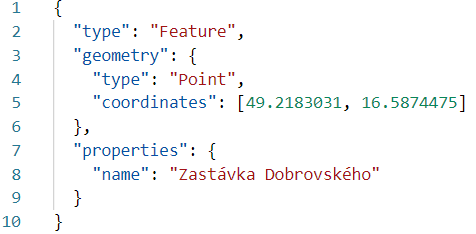
\includegraphics[width=0.7\textwidth]{obrazky/geojson_example.png}
    \caption{Příklad GeoJSON syntaxe}
    \label{geojson_example}
\end{figure}

\newpage
\section{Zobrazení získaných dát}
\label{olvsleaflet}
V sekci jsou rozebrány různé možnosti poskytnutí zobrazení dat uživateli, které jsou zváženy pro další vývoj.
\subsection{OpenLayers}
OpenLayers je knihovna napsaná v~JavaScriptu. Dle názvu lze poznat, že se nástroj pohybuje v~tzv. vrstvách (angl. \emph{Layers}). Různé vrstvy jsou navrženy pro různé typy zobrazení dat. Vrstvy umožňují jednodušší zobrazení uživateli, koncept lze vysvětlit na příkladu z~knížky \emph{OpenLayers 2.10 Beginner's Guide}: 
\begin{quote}
    Představte si dva lidi, kteří se dívají na mapu města. Jeden z~nich se zajímá o~autobusové trasy zatímco druhý má zájem o~cyklistické trasy. Místo vytváření dvou map lze vytvořit dvě vrstvy na jedné mapě a~následně si uživatel sám vybere, zda chce vidět pouze jednu nebo dokonce obě vrstvy naráz. \cite{openlayers2}
\end{quote}
Pro zobrazení dokáže knihovna zpracovat větší množství různých typů dat. Například může používat GML (angl. \emph{Geography Markup Language}), GeoJSON nebo v~ní lze také jednoduše zobrazit pole souřadnic jako různé útvary\,--\,mnohoúhelníky. Při definici je na výběr velké množství zdrojů samotného obrázku mapy, jako jsou například Google Mapy a~OpenStreetMap. \cite{openlayers3}
\subsection{Leaflet}
\label{leaflet}
Leaflet je volně dostupná knihovna napsaná v~JavaScriptu. Pomocí knihovny lze zobrazit
geografická data, např. GPS body na mapě. Tato mapa je externě zobrazena díky databázi
OpenStreetMap. Pro zlepšení uživatelského komfortu lze nastavit různé parametry, jako
např. úroveň přiblížení a~stylování objektů pomocí CSS. Syntaxe zápisu objektů do mapy
je definována pomocí výměnného formátu GeoJSON. \cite{leaflet}
\newpage
\section{Návrh získaní dat}
V~rámci práce bylo zváženo vytvoření mobilní aplikace. Samotný vývoj jednoduché aplikace pro sbírání polohy by nebyl časově náročný, ale aplikace by se nevyrovnala již existujícím alternativám bez vložení početného množství hodin a~práce. Proto byl  zvolen přístup využití již existující aplikace, kdy hlavní požadavek byl existence moderní mobilní aplikaci pro záznam dat. Dle průzkumu ze sekce~\ref{appcomparison} byla zvolena aplikace Strava. 

Pro získání uživatelských dat je doporučené využít volně dostupné API z~aplikace Stravy. Zde je jediná podmínka být registrovaný uživatel, následně má každý jednotlivec možnost si zaregistrovat vlastní API instanci pro svůj účet. Pro zaregistrování je potřeba mít připravený název, kategorii a~webovou adresu. Webová adresa nemusí být nutně platná, zde se dá vyplnit i~adresa lokálního serveru (angl. \emph{Localhost}).
API Strava generuje tzv. OAuth autorizační stránku po obdržení požadavku, ten musí mít validní parametry pro identifikaci registrované instance API. Uživatel je na této stránce srozuměn s~povoleními a~rámcem přístupu, které uděluje fitness aplikaci. Po úspěšné autorizaci dostává aplikace přístup
k datům uživatele. Tento proces je názorně zobrazen na obrázku~\ref{stravaauth}.~\cite{strava}

Strava API má omezenou režii, tj. 100 požadavků během 15 minut a~maximálně 1000 za 24 hodin. \cite{strava}

Pro potřeby bakalářské práce je toto množství požadavků dostačující, ovšem pro produkční použití by bylo potřeba vyjednat úmluvu se Stravou.
\begin{figure}[h]
    \centering
    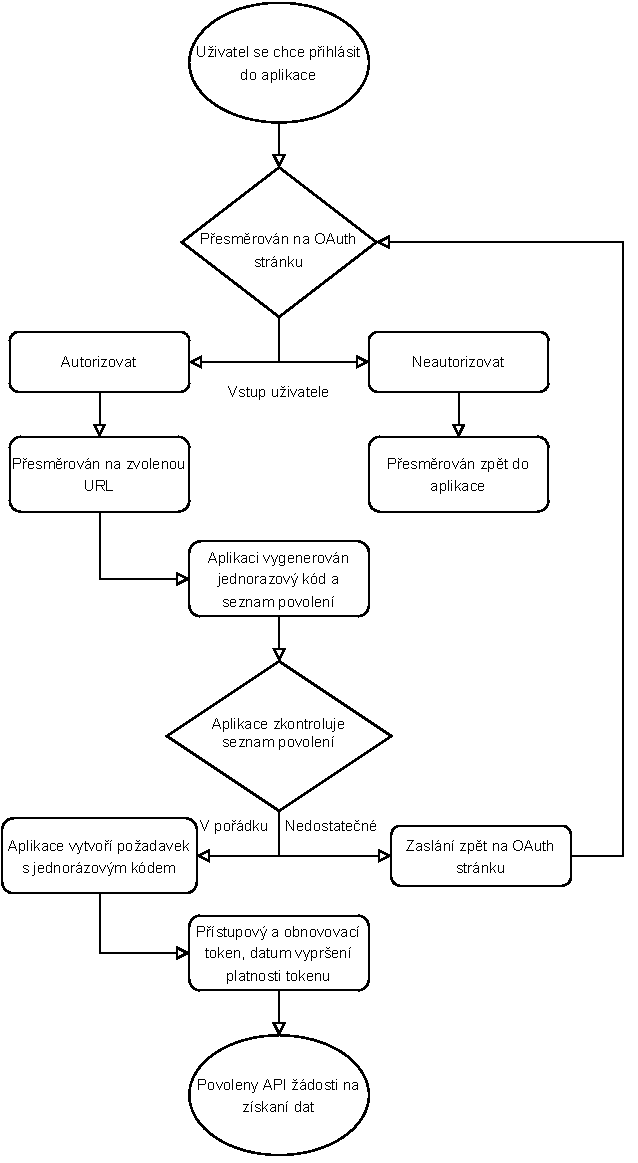
\includegraphics[width=0.75\textwidth]{obrazky/strava_auth.pdf}
    \caption{Diagram autorizace uživatele}
    \label{stravaauth}
\end{figure}
\clearpage
\section{Návrh uživatelského rozhraní}
\label{wireframes}
Po přístupu na webovou stránku uživatele uvítá přihlašovací obrazovka. Dle předešlých vysvětlení je možné k~autorizaci využít API Stravy. Na této stránce je z~daného důvodu nutné implementovat pouze elementy k~přesměrování.
Struktura aplikace bude rozdělena na 3 části\,--\,navigační menu vlevo, hlavička s~uživatelským jménem a~možností odhlášení. Zbytek stránek tvoří dynamicky se měnící obsah. Navigační menu se bude nacházet na levé straně aplikace, po najetí kursorem se rozevře a~zobrazí uživateli názvy jednotlivých webových stránek.
V hlavičce se bude vyskytovat název aplikace, uživatelské jméno a~tlačítko pro odhlášení. Po kliknutí na jméno nebo ikonku uživatele se zobrazí dodatečné funkce uživatelského účtu.
\subsubsection{Seznam aktivit}
Po úspěšném přihlášení uživatele bude první stránka seznam jeho aktivit. Zde bude mít uživatel možnost kliknout na jednotlivé aktivity, které se následně otevřou a~zobrazí uživateli trasu aktivity a~dodatečné informace. Každá aktivita také bude mít možnost smazání z~aplikace pomocí menšího tlačítka. Ve spodní části stránky se bude vyskytovat stránkování, což uživateli poskytuje možnost jednoduše procházet seznam jeho aktivit. Také si bude moci nastavit, kolik aktivit chce na jedné stránce zobrazit. Návrh této stránky je znázorněný na obrázku~\ref{wf:runs}.
\begin{figure}[h]
    \centering
    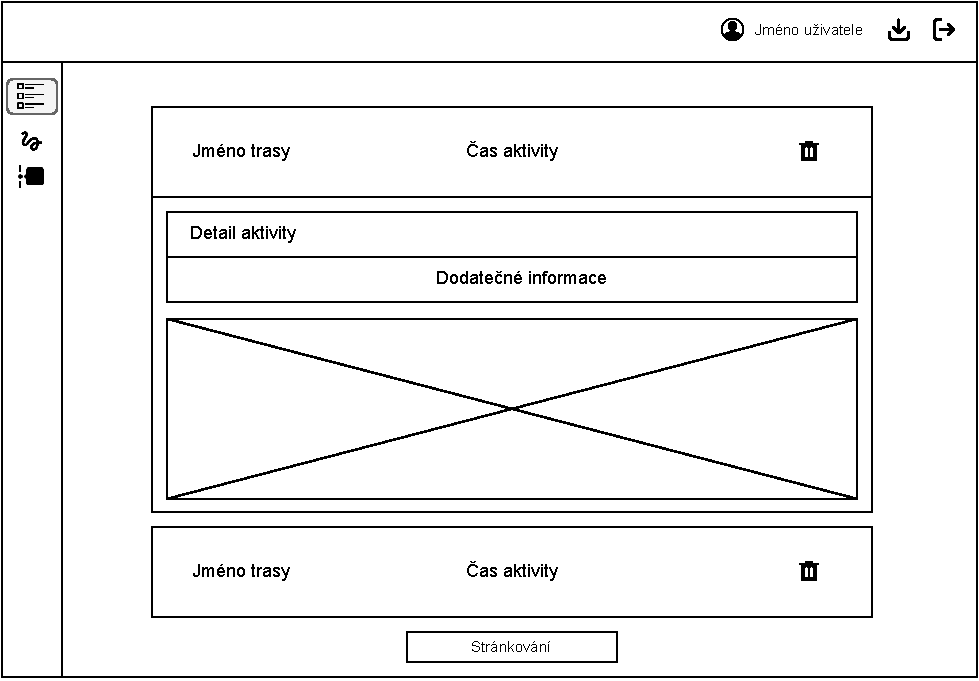
\includegraphics[width=1\textwidth]{obrazky/wf_activitylist.pdf}
    \caption{Uživatelské aktivity}
    \label{wf:runs}
\end{figure}
\newpage
\subsubsection{Zabrané území a~zobrazení filtrace tras}
Na stránkách \emph{Filtrované trasy} a~\emph{Zabrané území} si bude moci uživatel prohlédnout jeho zpracované data. Na stránce se musí vyskytovat komponent mapy, která uživateli zobrazí jeho data. Součástí stránky bude legenda, která od sebe odliší jednotlivé aktivity. Pro uživatelské pohodlí je vhodné implementovat různé způsoby přizpůsobení. Je vhodné barevně odlišit od sebe jednotlivé trasy a~viditelně zobrazit zabrané území. Přizpůsobením se může rozumět například změna barev jednotlivých tras, změna tloušťky hranic apod. Data v~legendě a~na hlavní mapě se budou lišit dle stránky, ke které uživatel přistoupí. Návrh stránky je vidět v~obrázku~\ref{wf:map}.
\vspace{1cm}
\begin{figure}[h]
    \centering
    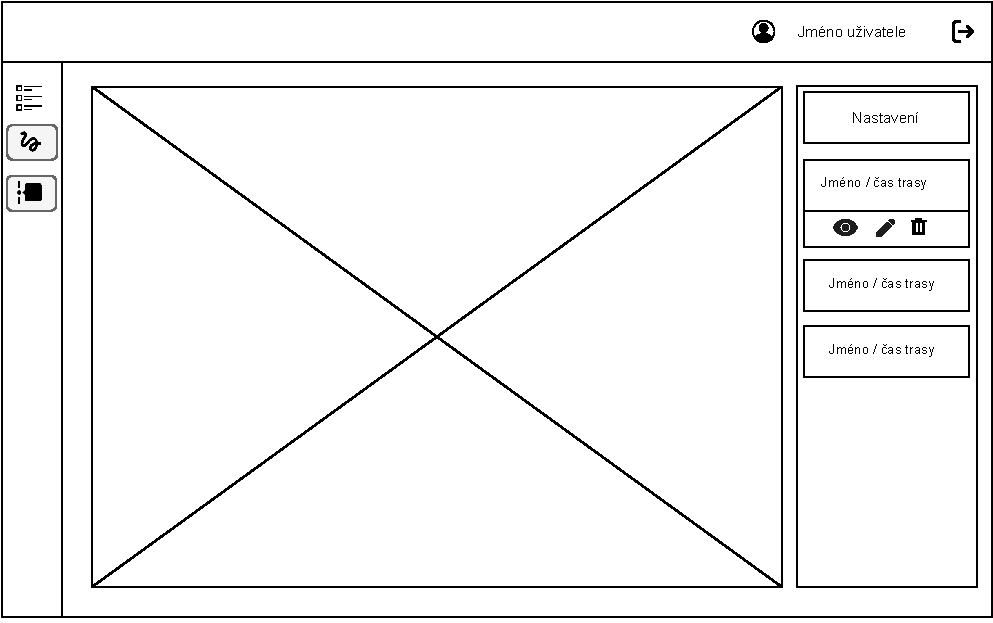
\includegraphics[width=1\textwidth]{obrazky/wf_map.pdf}
    \caption{Souhrn tras a~zabrané území}
    \label{wf:map}
\end{figure}
\newpage
\subsubsection{Responzivita aplikace}
Drtivá většina moderních webových aplikací musí počítat s~přístupem uživatelů pomocí mobilního telefonu. Je potřeba aby se aplikace přizpůsobila, pokud je šířka prohlížeče omezená. Obrázek~\ref{wf:mobilemap} popisuje například změnu navigačních menu do tzv. \emph{hamburgeru} a~dalšího elementu, který zobrazí uživatelské menu přizpůsobení zmíněné na minulé stránce.
\vspace{1cm}
\begin{figure}[h]
    \centering
    
\includegraphics[width=0.5\textwidth]{obrazky/wf_mobilemap.pdf}
    \caption{Zobrazení pro mobilní zařízení}
    \label{wf:mobilemap}
\end{figure}

\chapter{Implementace řešení}
\label{implement}
\section{Příprava serveru}
\label{serversetup}
Sekce popisuje části, které byly nutné připravit a~implementovat v~první fázi.
\subsection{Konfigurační soubor}
\label{config}
K bezpečnému uložení konfigurace je použit soubor \emph{appsettings.json}. Díky uložení většiny důležitých nastavení v~jednom souboru je lze v~budoucnu jednodušeji změnit a~není potřeba zasahovat přímo do zdrojového kódu aplikace. To se hodí například při změně adresy databáze apod. 

Soubor je načten v~C\# pomocí metody \texttt{builder.Configuration.AddJsonFile()} a~ následně se k~němu přistupuje pomocí DI (angl. \emph{Dependency Injection}), které je vysvětlené v~sekci~\ref{apiimplementation}. Následně je instance definovaná jako třída \emph{IConfiguration}.
Příklad struktury v~souboru appsettings.json:
\begin{verbatim}
    {
        "Strava": {
            "clientid": "72572",
        }
    }   
\end{verbatim}
V koncovém bodu se následně přistupuje k~objektům pomocí jeho cesty:
\begin{verbatim}
    Iconfiguration config;
    config["Strava:clientid"]
\end{verbatim}
Tímto způsobem jsou do souboru uloženy adresy pro připojení k~databázi, k~přístupu do Stravy nebo adresa frontendu.
\subsection{Vytvoření databáze}
\label{dbcreation}
Databáze je vytvořena pomocí tzv. \emph{Code First} přístupu. To znamená, že jsou vytvořeny objekty a~třídy a~podle nich vytvořené tabulky v~databázi. Za použití C\# byl využit pro tento proces EF (angl. \emph{Entity Framework}). EF poskytuje mapování relací objektů (angl. Object Relational Mapping) v~platformě .NET díky vytvoření konceptuálního modelu aplikační domény. Tento model popisuje vytvořené třídy a~objekty, které následně využívá pro vytvoření dotazů do databáze. V~minulosti EF fungoval na bázi vytvoření konceptuálního modelu pomocí reverzního inženýrství již existující databáze do souboru XML. Pro tento typ souboru bylo vytvořeno prostředí, ve kterém šlo model dále upravovat. Od doby vytvoření EF si vývojáři žádali o~možnost psát pouze kód a~ve verzi .NET 4.1 byl představen koncept \emph{Code First}. Při psaní \emph{Code First} je nutné si pouze definovat objekty a~třídy, které nejsou nutně specifické k~EF. Jedná se o~klasické C\# třídy. EF dokáže rozpoznat větší množství informací o~vaší zamýšlené databázi dle různých definic využitých v~těchto třídách. EF poskytuje další možnosti manuální konfigurace, což přijde vhod, pokud automatické generování nefunguje dle představ vývojáře, např. špatně mapované relace nebo typy sloupce. \cite{CodeFirst1,CodeFirst2}  
Po definování základních tříd a~objektů, které tvoří databázi je také potřeba definovat jednotlivé tabulky pro \emph{Entity Framework}. To se děje v~souboru \emph{AppDbContext}, tzv. \emph{Properties} definované v~této funkci poskytují přímý přístup z~aplikační vrstvy do databáze. Také lze zde pomocí metody \emph{OnModelCreating} definovat speciální vlastnosti relací a~tabulek, jako je například chování po smazání řádku v~tabulce. Jako příklad lze vzít třídu \emph{User}, ta je následně díky \emph{Entity Frameworku} přeložena a~v databázi je vytvořena tabulka \emph{Users}. Útržek kódu definice třídy \emph{User} v~C\#:   
\begin{verbatim}
    [Key]
    [DatabaseGenerated(DatabaseGeneratedOption.None)]
    [Required]
    public long Id { get; set; }
    public string Name { get; set; } = null!;
    [StringLength(50)] public string Username { get; set; } = null!;
    [StringLength(300)] 
    public string? AccessToken { get; set; }
    [StringLength(300)] 
    public string? RefreshToken { get; set; }
    public DateTime? AccessExpiresDate { get; set; }
    public DateTime LastUpdated { get; set; }
    public virtual List<UserActivity> Activities { get; set; } = new();
\end{verbatim}

Po zapsání definice entit se pomocí konzolového řádku spustí EF, který vygeneruje tzv. \emph{migraci}. Migrace popisují změny, které proběhly od poslední změny databázového modelu. EF porovnává současný model oproti snímku staršího modelu pro výpočet rozdílných objektů nebo entit. \cite{EFMigrations} 

Migrace se jménem PrvniMigrace by se přidala pomocí příkazu: 
\begin{verbatim}
    dotnet ef migrations add PrvniMigrace
\end{verbatim}
Následně pro aplikování změn do databáze se používá příkaz:
\begin{verbatim}
    dotnet ef database update
\end{verbatim}
\subsection{Implementace API}
\label{apiimplementation}
Základ API je definován v~souboru \emph{Program.cs}, pomocí syntaxe \emph{Minimal API}. To je nový framework uvnitř frameworku \emph{.NET 6} a~vyšší, který si dává za cíl minimalizaci množství psaného kódu. C\# Minimal Api využívá \emph{Dependency Injection} u~všech jeho koncových bodů. Funkce DI je poskytnout metodě všechny relevantní objekty, které potřebuje. Metoda samotná nehledá instance objektů, ale naopak jsou ji předány jako parametry. V~implementaci \emph{Minimal API} je třída \emph{builder.Services} je prostředník pro DI a~následně jsou do ní vložené nutné služby.
   
Jednoduché vysvětlení poskytuje otázka z~knížky Dependency Injection Principles, Practices, and Patterns\,--\,\uv{Jak vysvětlit Dependency Injection 5letému dítěti?} \cite{DI}:
\begin{quote}
    \uv{
        Pokud si zkusíš vzít jídlo z~ledničky pro sebe, je možné, že nastanou problémy. Můžeš nechat otevřené dveře ledničky, můžeš si vzít něco, co by tvoje mamka a~taťka nechtěli, aby jsi měl. Nebo také můžeš v~ledničce hledat něco, co tam vůbec není nebo už je prošlé.
        Místo hledání je lepší říci: \uv{Potřebuji nějaké pití k~obědu} a~poté se rodiče postarají o~to, aby jsi měl něco k~pití.
    }
\end{quote}
\noindent Do DI je přidáno několik dalších služeb, např. \emph{Hangfire}, který je dále probraný v~sekci~\ref{transformData}. Za zmíňku stojí nastavení CORS (angl. \emph{Cross-Origin Resource Sharing}). CORS dovoluje prohlížeči klienta vytvářet a~posílat požadavky na API mezi různými doménami. Toto se může hodit v~případě, že API je hostované na jiném serveru a~případně doméně než samotný server pro frontend. Pokud by tento případ nastal, požadavky by byly automaticky zablokovány prohlížeči a~uživatelé by nemohli komunikovat s~API. Zde se objevuje koncept CORS, který tuto komunikaci povoluje. \cite{CORS}

Webová aplikace byla po dobu testování a~vývoje spouštěna na lokálním serveru na portu 3000, zatímco API běželo na portu 7040. Už toto nastavení jiných portů vyžaduje povolení CORS. Pro přidání CORS do služeb v~C\# \emph{Minimal API} se využívá metoda \texttt{builder.Services.AddCors()}.
Příklad konfigurace pro povolení CORS na lokálním serveru:
\begin{verbatim}
    builder.Services.AddCors(policyBuilder =>
        policyBuilder.AddPolicy("AllowLocalhost", x=> 
            x.AllowAnyMethod()
             .AllowAnyHeader()
             .AllowCredentials()
             .SetIsOriginAllowed(origin => 
                new Uri(origin).Host == "localhost")
             ));
\end{verbatim}
\noindent Pomocí \emph{builder.Services.AddAuthentication()} se zde také nastavuje využití souborů cookie pro autentizaci, dále probrané v~sekci~\ref{userAppStravaConnection}. 
\subsection{Koncové body}
Koncové body představují základ komunikace mezi API a~klientem. Každý koncový bod definuje svoji URL cestu, ke které klient přistupuje pomocí tzv. HTTP (angl. \emph{Hypertext Transfer Protocol}) požadavků. Ty jsou dále vysvětleny v~sekci~\ref{httpreq}. \emph{Minimal API} umožňuje mapovat funkce přímo na koncový bod. Po přijetí požadavku se API podívá zdali existuje koncový bod s~definovanou URL cestou a~pokud ano, tak se spustí namapovaná funkce. Tento způsob plně podporuje \emph{Dependency Injection}, předávání parametrů pomocí URL parametrů nebo také jako součástí těla požadavku. Při definici koncového bodu lze také definovat zdali uživatel musí být přihlášen nebo mít specifickou roli v~systému. Pokud klient nesplňuje dané přístupové povolení, tak se automaticky odepře přístup.    

\noindent Příklad mapování koncového bodu: 
\begin{verbatim}
    app.MapPost("/api/register", AuthRepository.Register)
        .AllowAnonymous();    
\end{verbatim}
A následně \emph{Minimal API} využije \emph{Dependency Injection} pro předání následujících parametrů: 
\begin{verbatim}
    public static async Task<IResult> Register
        (AppDbContext dbContext, HttpClient httpClient, 
        HttpContext context, IConfiguration config, 
        IBackgroundJobClient backgroundJobs,
        [FromQuery] string state, [FromQuery] string code, 
        [FromQuery] string scope)
    {...}
\end{verbatim}
\noindent Obdobným způsobem jsou definovány všechny koncové body v~API, které klient potřebuje.
\section{Naplnění statických dat}
V sekci je popsána příprava a~způsob získání dat nutných k~funkci aplikace v~pozdější fázi.
\subsection{Overpass pro OSM}
\label{overpass}
\emph{Overpass} je API, které dovolí svým klientům přistupovat k~datům uložených v~databázi~OSM pomocí speciálních výrazů, tzv. \emph{query}. Existuje množství oficiálních serverů, které jsou veřejně přístupné. Servery lze využít v~případě malé režie, tj. jsou omezeny zhruba na 10000 dotazů denně.~\cite{OSMAPI}

Pro potřeby práce byl vytvořen virtuální stroj v~portálu \emph{Azure}. V~době vytváření toho virtuálního stroje bylo pro licenci \emph{Azure for Students} dostupný pouze region v~Austrálii. To značně omezuje rychlost aplikace, v~kombinaci s~levnější volbou procesorových jader mají veškeré požadavky následně okolo 500~milisekund zpoždění při spuštění lokální verze aplikace z~\emph{Dockeru}. Úplný návod pro spuštění aplikace pomocí \emph{Dockeru} se nachází v~příloze~\ref{startapp}. \cite{azure}. 

Pro instalaci \emph{Overpass} API na virtuální stroj bylo postupováno podle oficiálního návodu pro vytvoření vlastní instance serveru\footnote{Více informací na: \url{https://wiki.openstreetmap.org/wiki/Overpass_API/Installation}.}. V~rámci instalace API byl zprovozněn \emph{Apache} server, který zprostředkuje přístup k~databázi OSM.~\cite{apache}

\subsubsection{Příprava OSM dat}
K naplnění databáze byl využit soubor OSM dat pro Českou Republiku dostupný ze serverů VUT FIT\footnote{OSM data pro ČR: \url{ https://osm.fit.vutbr.cz/extracts/czech_republic/}.}. Ze souboru byly následně extrahovány data pomocí skriptu \emph{Osmosis}\footnote{Osmosis dostupné~z: \url{https://wiki.openstreetmap.org/wiki/Osmosis}.}. Na výstupu jsou data, která zobrazují pouze různé cesty v~Brně a~okolí.

Soubor je ořezaný o~informace infrastruktur a~dalších nepodstatných prvků pomocí příkazu:

\begin{verbatim}
    ./osmosis --read-pbf czech_republic-2021-10-23.osm.pbf  
              --tf accept-ways highway=* 
              --tf reject-ways highway=sidewalk,crossing 
              --tf reject-relations 
              --bounding-box 
                top=49.25589126316103 left=16.475088825520327
                bottom=49.1459949173186 right=16.7047932397780
              --used-node --write-xml brno.osm
\end{verbatim}
\subsection{Příprava databáze serveru}
\label{SQLDB}
Myšlenka přístupu k~regionům je tvořena na principu uložení jednotlivých středů regionů do databáze společně s~body, které ohraničují území a~tvoří Voroného region. Zdroj dat je soubor z~předešlého odstavce, následně jsou jeho data dále extrahována pomocí python skriptu \texttt{extract\_nodes\_from\_osm.py}. Soubor zkopíruje jméno vstupního souboru a~přidá mu příponu \texttt{\_nodes}. Na výstupu jsou čisté souřadnice všech středů regionů, jako jsou např. silnice, ulice a~cesty. Stejný princip by bylo možné využít i~globálně, aby aplikace nebyla omezena pouze na oblast Brna. Největší problém jsou zde potom hardwarová omezení, jako je např.~kapacita úložiště v~portálu Azure a~rychlost prohledávání SQL databáze. 

Další krok spočívá ve vypočítání hranic Voroného regionů. Díky skriptu \texttt{run\_voronoi.py} byly všechny body ze souboru \texttt{*\_nodes.txt} podrobeny funkci \emph{Voronoi} z~knihovny \emph{Scipy}, zmiňované v~sekci~\ref{voronoi}. Na výstupu je vytvořen soubor \texttt{*\_nodes\_regions.txt}, který obsahuje jako první dvě položky zeměpisné souřadnice středu regionu a~následně řetězec znaků jako pole hraničních souřadnic Voroného regionu. Dělitel sloupců byl nastavený jako znak \uv{;}. Počet Voroného regionů pouze pro Česko přesáhl 9,5~milionu. To znamená, že i~do databáze samotné by bylo následně vloženo 9,5~milionu řádků. Z~důvodu implementace databáze na online placeném portálu \emph{Azure} byl tento soubor dále zmenšen pro potřeby bakalářské práce pouze na oblast Brna a~okolí. To je ve výsledku necelých 200~tisíc řádků. Značně to ulevilo rychlosti celé aplikace při zpracování aktivit, přičemž další oblasti by nebyl problém v~budoucnu vložit. Samotný proces vložení byl proveden pomocí nástroje \emph{Microsoft SQL Server Management Studio}\footnote{SQL Server Management studio dostupné z: \url{https://docs.microsoft.com/en-us/sql/ssms/download-sql-server-management-studio-ssms?view=sql-server-ver15}}.

Příklad jednoho řádku z~exportovaného souboru \texttt{*\_nodes\_regions.txt}:
\begin{verbatim}
            16.5001211;49.1761032;'[16.49919818031525,49.174517706363304],
            [16.500758940325838,49.17438858468905],
            [16.500975032570768,49.17589229164807],
            [16.49952847265777,49.17635098941457],
            [16.499449708003834,49.176045363691514],
            [16.49919818031525,49.174517706363304]'
\end{verbatim}
\subsubsection{Vložení regionů do databáze}
Po navázání připojení s~databází v~aplikaci \emph{SQL Server Management Studio} je potřeba otevřít konkrétní model databáze, který obsahuje vytvořené tabulky. Pravým tlačítkem se otevře kontextové menu a~pod tlačítkem \emph{Tasks} se nachází možnost \emph{Import Data}. Toto lze vidět na obrázku~\ref{studio_1}. Po otevření dialogu je nutno zvolit typ zdroje. V~tomto případě se jedná o~\emph{Flat File Source}. Jelikož soubor \emph{VoronoiRegion.src} neobsahuje názvy sloupců, je potřeba relevantní zaškrtávací políčko odškrtnout. Následně je nutno v~liště správně navolit oddělovací znaky. Sloupce jsou rozděleny pomocí znaku \uv{:} a~řádky pomocí \uv{\{LF\}}. Pod lištou \emph{Advanced} je doporučeno nastavit typ zdrojové proměnné. V~případě bakalářské práce se jedná o~typ \emph{double-precision float [DT\_R8]} pro první dva sloupce a~\emph{text\_stream [DT\_TEXT]} pro třetí sloupec. V~\emph{Preview} lze jednoduše zkontrolovat, zda rozdělení dat na sloupce a~řádky funguje dle očekávání. Správně rozdělení do sloupců je znázorněno na obrázku~\ref{studio_2}. V~poslední řadě je potřeba sloupce správně namapovat. Jelikož je databáze vytvořena pomocí \emph{Code First} přístupu, tak se vkládají data již do existující tabulky \emph{StaticRegions}. Obrázky zobrazující vložení dat jsou k~nalezení v~příloze~\ref{sqlserverpictures}.
\newpage
\section{Registrování API pro Stravu}
\label{registerstrava}
Každý registrovaný uživatel má možnost si ve Stravě zaregistrovat vlastní aplikaci pro přístup k~Strava API. To je dostupné na stránce \url{https://www.strava.com/settings/api}, v~kategorii \uv{My API Application}. Tuto stránku lze vidět na obrázku~\ref{myapiapp}.

Díky tomuto procesu je umožněn přístup k~uživatelským datům z~databáze Stravy. Každá aplikace pak má přidělené jednoznačné identifikační prvky:
\begin{itemize}
    \item Client Id.
    \item Client Secret.
\end{itemize}
Tyto parametry Strava využívá pro autentizaci uživatelské aplikace do Stravy. Díky nim dokáže Strava přesně říci, jak velkou režii mají jednotlivé aplikace a~k jakým datum přistupují. 
\vspace{1cm}
\begin{figure}[h]
    \centering
    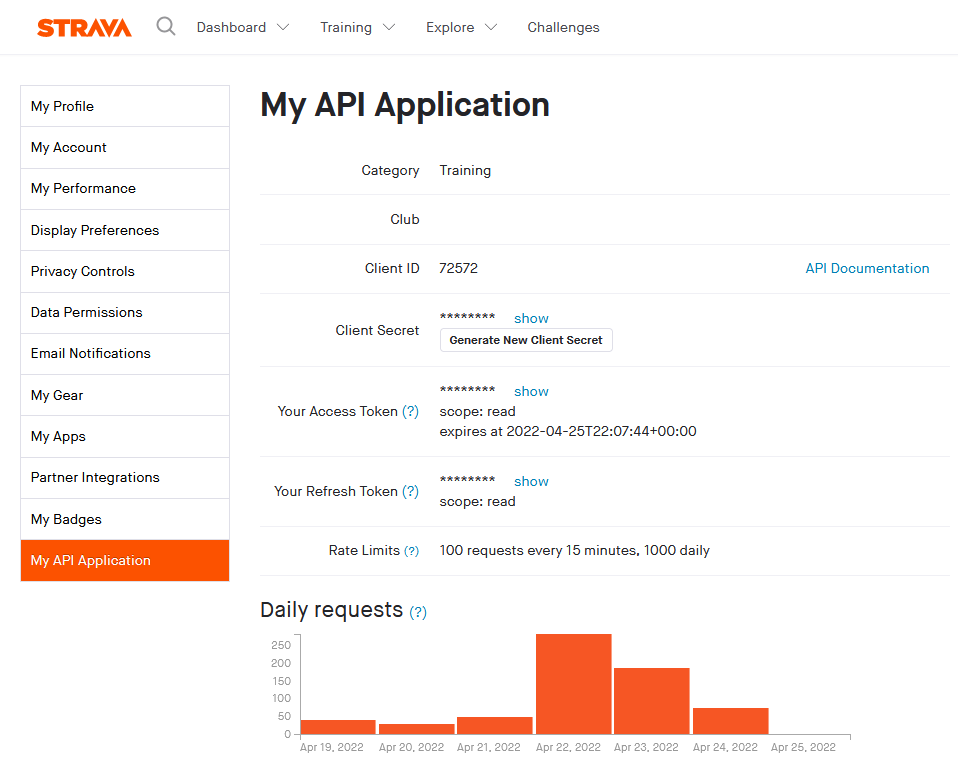
\includegraphics[width=1\textwidth]{obrazky/myapiapp.png}
    \caption{Sekce My Api Application na stránce Strava}
    \label{myapiapp}
\end{figure}
\newpage
\section{Propojení uživatele, aplikace a~Stravy}
\label{userAppStravaConnection}
V sekci je detailně probrané téma implementace navázání spojení a~přístupu k~uživatelským datům.
\subsection{Propojení z~pohledu uživatele}
Po kliknutí na tlačítko \uv{Přihlásit} je uživatel přesměrován na stránku Stravy, kde se přihlásí do svého účtu. V~případě, že je již přihlášen, je mu zobrazena stránka s~potvrzením povolení přístupu.
Výběr k~jednotlivým oprávněním se uživateli zobrazí ve formě zaškrtávacích políček. Doporučené povolení je čtení všech aktivit, aplikace nežádá žádný zápis do Stravy. 

Po udělení oprávnění mapové aplikaci je uživatel přesměrován na seznam aktivit. Pokud se uživatel přihlásil do aplikace poprvé, tak se na straně API začnou zpracovávat uživatelovi aktivity, viz sekce~\ref{transformData}. Diagram komunikace fitness aplikace s~API aplikace Stravy je zobrazený na obrázku~\ref{stravaauth}.

\subsection{Propojení z~pohledu API}
Po přijetí požadavku ze strany webové aplikace je vygenerována adresa URL. Jako parametry jsou dále přidány identifikační prvky pro Stravu\footnote{Dokumentace pro autentizaci do Stravy: \url{https://developers.strava.com/docs/authentication/\#tokenexchange}}:
\begin{itemize}
    \item URL Stravy.
    \item Client ID.
    \item URL pro přesměrování (angl. \emph{Redirect\_uri}).
    \item Požadované povolení (angl. \emph{Scope}).
\end{itemize}
Následná URL je předána zpátky klientovi jako odpověď a~klient se přesměruje.
Šablona URL jako příklad pro komunikaci:
\begin{verbatim}
    https://www.strava.com/oauth/authorize?client_id=72572
    &response_type=code
    &redirect_uri=https://localhost:3000?register=/api/register
    &scope=profile:read_all,activity:read_all
\end{verbatim}
Jakmile uživatel autorizuje aplikaci přístup na stránce Stravy, tak je klient přesměrován na dříve zadanou URL. Po autorizaci Strava dále přidává do URL několik parametrů:
\begin{itemize}
    \item \emph{Code} -- jednorázový kód pro získání obnovovacího a~přístupového tokenu.
    \item \emph{Scope} -- přístup udělený uživatelem.
\end{itemize}
Klient zpracuje tyto parametry z~URL a~dále je předá do API pomocí koncového bodu. Zde je následně použít parametr \emph{Code} pro získání obnovovacího a~přístupového tokenu ze Stravy. Toto chování požadavků a~odpovědí je součástí protokolu \emph{OAuth 2.0}\footnote{OAuth online dokumentace: \url{https://oauth.net/2/}}.

\subsubsection{OAuth 2.0}
\label{oauth}
OAuth je standardní protokol pro autorizaci. Cílem protokolu je jednoduchý přístup k~autorizaci při zachování integrity a~bezpečnosti uživatelských dat. Díky tomuto protokolu je možné přistupovat k~uživatelským datům bez nutnosti předávání citlivých uživatelských dat, jako jsou přihlašovací jméno a~heslo.
Přístupové tokeny mají standardně dobu platnosti. Do doby vypršení lze za pomocí těchto tokenů posílat požadavky na API\,--\,v~případě fitness aplikace se jedná o~API aplikace Strava. Díky těmto přístupovým tokenům Strava dokáže rozpoznat, zdali uživatel doopravdy udělil požadované aplikaci přístup ke svým datům a~následně vygeneruje odpověď. 
V~případě, že vyprší doba platnosti přístupového tokenu, tak API posílá požadavek pro nový přístupový token za pomocí obnovovacího tokenu. Tento protokol také umožňuje uživateli lehce zrušit přístup ke svému účtu cizí aplikaci. To může přijít v~hod v~případě, že uživatel nemá potřebu aplikaci nadále využívat nebo dojde k~narušení bezpečnosti jeho účtu.~\cite{OAuth}

Na množství stránek lze vidět tlačítka \uv{Přihlásit pomocí Google} nebo \uv{Přihlásit pomocí Facebooku}. Tyto tlačítka v~pozadí fungují na principu \emph{OAuth 2.0}. Pro přihlášení do mapové aplikace je tento protokol také využit. Po udělení přístupu aplikace k~uživatelským datům je vytvořena kopie uživatelského účtu v~databázi aplikace, také je k~účtu uložen přístupový a~obnovovací token. V~poslední řadě se začnou stahovat uživatelské aktivity ze Stravy. Proces zpracování je dále objasněn v~sekci~\ref{transformData}. 

\subsubsection{Opakované přihlášení}
Pro vyvrácení nutnosti přihlášení uživatele při každém navštívení stránky byla řešena otázka, zdali využívat soubory cookie (angl. \emph{Cookie-based Authentication}) nebo JWT\footnote{JWT online dokumentace: \url{https://jwt.io/}} (angl. \emph{JSON Web Token}). \cite{CookieVsJWT}

JSON Web Token je standardizovaný způsob přenosu informací mezi dvěma objekty během autorizace. Jakmile je uživatel přihlášen, každý následující požadavek v~sobě obsahuje JWT, na což reaguje API a~zpřístupní uživateli koncové body. Věrohodnost je doložena elektronickým podpisem. Mohou být podepsány pomocí algoritmu využívající tzv. \emph{hashování}. Při hashování dat pomocí dané funkce je vždy vytvořený stejný řetězec znaků. Z~výsledného řetězce nelze zpětně zjistit vstupní data. Další možnost pro zajištění věrohodnosti je využití veřejného a~soukromého klíče. Z~obecného hlediska je JWT modernější způsob, který je složitější na implementaci, ovšem bezpečnější a~má lepší škálovatelnost. JWT se skládá z~hlavičky, dat a~podpisu. Hlavička se většinou skládá ze dvou částí\,--\,první popisující typ tokenu a~druhá část si ukládá informaci o~použitém podepisovacím algoritmu. V~datové části se vyskytují nároky (angl. \emph{Claims}), díky nim si klient dokáže i~uložit role uživatele systému, případně i~další informace. Na výstupu je řetězec znaků oddělený tečkami, který je zašifrovaný pomocí tajného klíče. \cite{CookieVsJWT, JWT}

HTTP Cookies jsou základním kamenem moderního internetu. Jsou to malé textové soubory uložené na straně uživatele, které obsahují data. Při využívání souborů cookie je jedna z~největších obav CSRF (angl. \emph{Cross-site Request Forgery}) útok. Funkce prohlížeče při otevření webové stránky je poslání všech relevantních cookies právě pro danou stránku. Tento útok pracuje na bázi přesměrování uživatele a~využití tohoto chování. Při úspěšném útoku jsou následně vytvořeny zfalšované požadavky na API pomocí cizí identity. \cite{Cookies, CSRF}

CSRF útok by ovšem pro fitness aplikaci neměl velký význam. Aplikace nemá práva zasáhnout do dat, které jsou uloženy v~databázi Strava. V~podstatě největší škodu, kterou útočník může napáchat je smazání učtu v~mapové aplikaci. Pro potřeby aplikace byla tedy zvolena technologie souborů cookie. Po přihlášení klienta je do prohlížeče následně vložena tzv. \emph{Session Cookie} obsahující identifikační řetězec. Tato cookie nemá nastavenou expirační dobu, co má za následek, že aplikace si pamatuje přihlášeného uživatele, dokud se uživatel manuálně neodhlásí. 

\subsection{Načtení dat}
\label{getData}
Po získání přístupového a~obnovovacího tokenu API začne načítat uživatelské informace.
Strava nazývá uživatelské trasy jako aktivity. Po vyslání požadavku dostává API jako odpověď jednoduchý seznam uživatelských aktivit\footnote{Strava API dokumentace seznam aktivit: \url{https://developers.strava.com/docs/reference/\#api-Activities-getActivityById}}. Tento seznam a~základní informace o~uživateli jsou ihned předány zpět klientovi. API dále prochází jednotlivé aktivity a~vytváří požadavky na tok aktivity (angl. \emph{Activity Stream})\footnote{Strava API dokumentace toku aktivity:  \url{https://developers.strava.com/docs/reference/\#api-Streams-getActivityStreams}}. Jednotlivým požadavkům je přidán parametr \emph{Keys} s~hodnotou \emph{Latlong}. To způsobí, že odpověď na požadavek je pouze pole souřadnic uživatelské aktivity. Následně jsou požadavky asynchronně poslány. Odpověď je uložena do databáze aplikace a~začne zpracování dat.

\section{Zpracování dat}
\label{transformData}
První část sekce obsahuje obecné informace o~zpracování dat v~pozadí API pomocí knihovny \emph{Hangfire}\footnote{Dokumentace Hangfire: \url{https://docs.hangfire.io/en/latest/}}. Následně je popsána tématika filtrování pomocí společné navštívené cesty. Poslední část řeší problematiku využití Voroného diagramu k~zabírání území uživatelem. 
\subsection{Zpracování v~pozadí}
Při vytváření aplikace nastala otázka škálování. Zpracování dat je velice náročná procesorová operace, která zabere větší množství času. To má za následek vysoké využití serveru a~následné omezení jeho funkčnosti. Otázka nastala, protože když byl server vytížený tak API server odpovídal na požadavky s~větším zpožděním. Z~dříve zmíněných důvodů byla využita služba \emph{Hangfire}.
\subsubsection{Hangfire}
Hangfire je široce dostupná služba. Lze ji používat v~.NET projektech, ASP.NET webových aplikacích, ale i~webových aplikacích jiného typu. Dále podporuje konzolové aplikace nebo i~služby Windows. Služba Hangfire vytváří úlohy běžící v~pozadí pomocí vláken. Úlohy mají několik různých typů:
\begin{itemize}
    \item Jednorázové (angl. \emph{Fire-and-forget}).
    \item Opakované (angl. \emph{Recurring}).
    \item Opožděné (angl. \emph{Delayed}).
\end{itemize}
Práce v~pozadí může být nastavena na opakované volání metod v~rozmezí vteřin, hodin až dní. Není potřeba vytvářet nové statické nebo instanční metody, Hangfire využívá již implementované metody. Použití Hangfire pomáhá se škálováním a~perzistencí aplikace. Pro zachování perzistence Hangfire využívá trvalé uložiště, to umožňuje vytvořeným úlohám přetrvat restarty nebo výpadky serveru. Trvalé uložiště můžou být např. SQL Azure nebo SQL Server. Úlohy jsou zpracovány pomocí Hangfire serveru. Server je implementován jako soubor vláken, která vyzvedávají úlohy z~uložiště. Server se také stará o~udržování čistého uložiště a~odstraňuje zastaralá data. \cite{Hangfire}

\subsubsection{Implementace Hangfire v~C\#}
Hangfire se do koncových bodů vkládá pomocí \emph{Dependency Injection}. Konkrétně pomocí třídy \emph{IBackgroundJobClient}.
    
\noindent Pro využití Hangfire musí metody být serializovatelné. To je hlavně z~důvodu ukládání dat do trvalého uložiště. V~praxi to znamená, že parametry metod nesmí být objekty, ale pouze jejich unikátní identifikátory. Pro každý jednotlivý úkol je nutno vytvořit novou instanci. V~případě, že by se toto nedělo, docházelo by k~problémům s~\emph{Garbage Collector} v~C\#, kdy reference na databázi může být uklizena dříve, než je úkol dokončen.
Pro proces instanciace je vytvořena třída \emph{ProcessActivityClass}. Následně jsou v~ní implementované metody pro filtrování (průměrování) cest a~přiřazení Voroného regionů uživateli. 
Příklad předávání pomocí identifikátorů: 
\begin{verbatim}
    public async Task RunAveraging(long activityId, long userId){...}
\end{verbatim}
Zde je místo odkazu na třídu aktivity a~uživatele předáno pouze jejich unikátní ID a~to je následně vyhledáno v~databázi.
\subsection{Filtrování cest}

Nejprve je potřeba zprůměrovat cestu v~rámci sebe sama v~případě, že v~jedné cestě uživatel projde stejnou trasu dva a~vícekrát. Z~původní cesty se vytvoří kopie, následně je vybrán první bod a~je prohledán zbytek této cesty. Po vybrání všech bodů, které jsou vzdáleny méně jako 15~metrů, je provedeno zprůměrování jejich souřadnic a~následně je přepsána jejich hodnota v~kopii trasy.  

\subsubsection{Vzdálenost souřadnice}
Souřadnice jsou objekty třídy \emph{RouteCoordinate}, která má instanční metodu \emph{GetDistanceTo}. Ta bere jako parametr druhý objekt třídy \emph{RouteCoordinate} a~následně vypočítá vzdálenost podle \emph{Haversine formula}\footnote{Výpočet vzdálenosti dle Haversine formule:
\url{https://www.movable-type.co.uk/scripts/latlong.html}}.

Ukázka implementace \emph{Haversine formule} v~C\# ze třídy \emph{RouteCoordinate}:
\begin{verbatim}
        public double GetDistanceTo(RouteCoordinate other)
        {
            double R = 6371e3;
            double num1 = Latitude * (Math.PI / 180.0);
            double num2 = other.Latitude * (Math.PI / 180.0);
            double d1 = (Latitude-other.Latitude) * (Math.PI / 180.0);
            double d2 = (Longitude-other.Longitude) * (Math.PI / 180.0);
            double a = Math.Sin(d1 / 2) * Math.Sin(d1 / 2) +
                       Math.Cos(num1) * Math.Cos(num2) *
                       Math.Sin(d2 / 2) * Math.Sin(d2 / 2);
            double c = 2 * Math.Atan2(Math.Sqrt(a), Math.Sqrt(1 - a));
            return R * c;
        }
\end{verbatim}


\subsubsection{Optimalizace}
V~případě průměrování mezi dvěma cestami existuje optimalizace. Třída \emph{RouteCoordinate} má relaci na pole objektů třídy \emph{CoordinateIndexes}. Tyto objekty jsou jednotlivé indexy všech dalších souřadnic v~rámci jedné cesty, které byly pod prahem\footnote{\,Prah = maximální vzdálenost dvou bodů.} algoritmu průměrování. A~tedy jsou to všechny souřadnice, které mají stejnou hodnotu zeměpisné šířky a~délky. Z~důvodu použití SQL databáze se zde jedná o~instanci třídy. V~jiných případech použití by tato třída šla nahradit jako pole čísel.

Z~důvodu způsobu zobrazení tras není možné lehce odstranit nadbytečné souřadnice. V~případě odstranění indexů by cesta měla nelineární průchod a~bylo by nutné složitě iterovat skrze pole \emph{CoordinateIndexes} a~upravovat všechny zasažené indexy. Náročnost zmíněného prohledávání je příliš vysoká.

\subsubsection{Filtrace cesty}
V~první části se průměruje cesta sama mezi sebou. Pokud se při iteraci objeví skupina souřadnic, která se nachází pod prahem, do objektu první souřadnice se uloží relace na novou instanci třídy \emph{CoordinateIndexes}. Tato instance je naplněna dříve zmíněnou skupinou souřadnic. Všechny souřadnice jsou také přepsány na stejnou zeměpisnou šířku a~délku. 

Po dokončení průměrování cesty samo sebou začne API postupně průměrovat všechny současné již alespoň jednou zprůměrované trasy. V~případě, že je nalezena alespoň jedna skupina souřadnic, která se nachází pod prahem průměrování, tak jsou dotyčné aktivity zařazeny do relace skupiny. Tato relace je v~budoucnu použita pro chytré přepočítávání aktivit v~případě odebrání (smazání) aktivity z~účtu aplikace. 

Postup algoritmu průměrování dvou cest je obdobný průměrování jedné cesty. Algoritmus iteruje přes dvě cesty. Pokud se při iteraci skrze druhou cestu některý z~bodů nachází pod prahem, je uložen do pomocného pole. Když algoritmus dosáhne konce druhé cesty, podívá se na pomocné pole a~vytvoří průměrnou hodnotu ze všech nalezených souřadnic. Zde se také dívá na pole \emph{CoordinateIndexes} všech souřadnic, které byly označeny jako pod prahem. Všechny indexy, které jsou v~tomto poli, jsou následně označený jako zkoumané a~dále je při iteraci algoritmus ignoruje. Také jsou souřadnice na těchto indexech upraveny dle nové zprůměrované zeměpisné šířky a~délky. 

Názorná ukázka výstupu filtrace dvou cest je viditelná na obrázcích~\ref{filter_routeA} a~\ref{filter_routeB}. Po dokončení filtrace jsou následně zprůměrované do jedné cesty, viditelné v~obrázku~\ref{filter_routeAB}.
\newpage
\subsubsection{Detaily implementace}
Pseudokod třídy \emph{RouteCoordinate}:
\begin{verbatim}
    double Šířka,
    double Délka,
    bool Centrovaná,
    CoordinateIndexes[] Indexy,
    Vzdálenost(RouteCoordinate souřadnice)
\end{verbatim}
Pseudokód algoritmu:
\begin{verbatim}
    Na vstupu pole: cestaA, cestaB
    Měj pole: IndexyAGlobal, IndexBGlobal
    podPrahem = false, Prah = 15
    Dokud indexA < délka(cestaA):
        souřadniceA = cestaA[indexA]
        Měj pole: IndexyvIteraci, stejnáŠířka, stejnáDélka
        
        Dokud indexB < délka(cestaB):
            souřadniceB = cestaB[indexB]
            Pokud indexA v IndexyAGlobal:
                break;
            Pokud indexB není v IndexyBGlobal:
                vzdalenost = souřadniceA.Vzdalenost(souřadniceB)
                Pokud Vzdalenost < Prah:
                    podPrahem = true
                    Přidej souřadniceB.Šířka do stejnáŠířka
                    Přidej souřadniceB.Délka do stejnáDélka
                    Přidej souřadniceB.Indexy do IndexyvIteraci
                    Přidej indexB do IndexyvIteraci
                    Přidej indexB do IndexyBGlobal
            Pokud indexB je délka(cestaB)-1:
                Přidej souřadniceA.Šířka do stejnáŠířka
                Přidej souřadniceA.Délka do stejnáDélka
                
                Projdi indexy v souřadniceA.Indexy a~přepiš cestaA 
                dle stejnáŠířka.průměr() a~stejnáDélka.průměr()
                
                Projdi indexy v souřadniceB.Indexy a~přepiš cestaB 
                dle stejnáŠířka.průměr() a~stejnáDélka.průměr()
                
                Přidej indexA do IndexyAGlobal
                přidej souřadniceA.Indexy do IndexyAGlobal
            Zvyš indexB
        Zvyš indexA
    Vrať podPrahem
\end{verbatim}
\newpage

\begin{figure} [h]
\centering
\begin{subfigure}
  \centering
  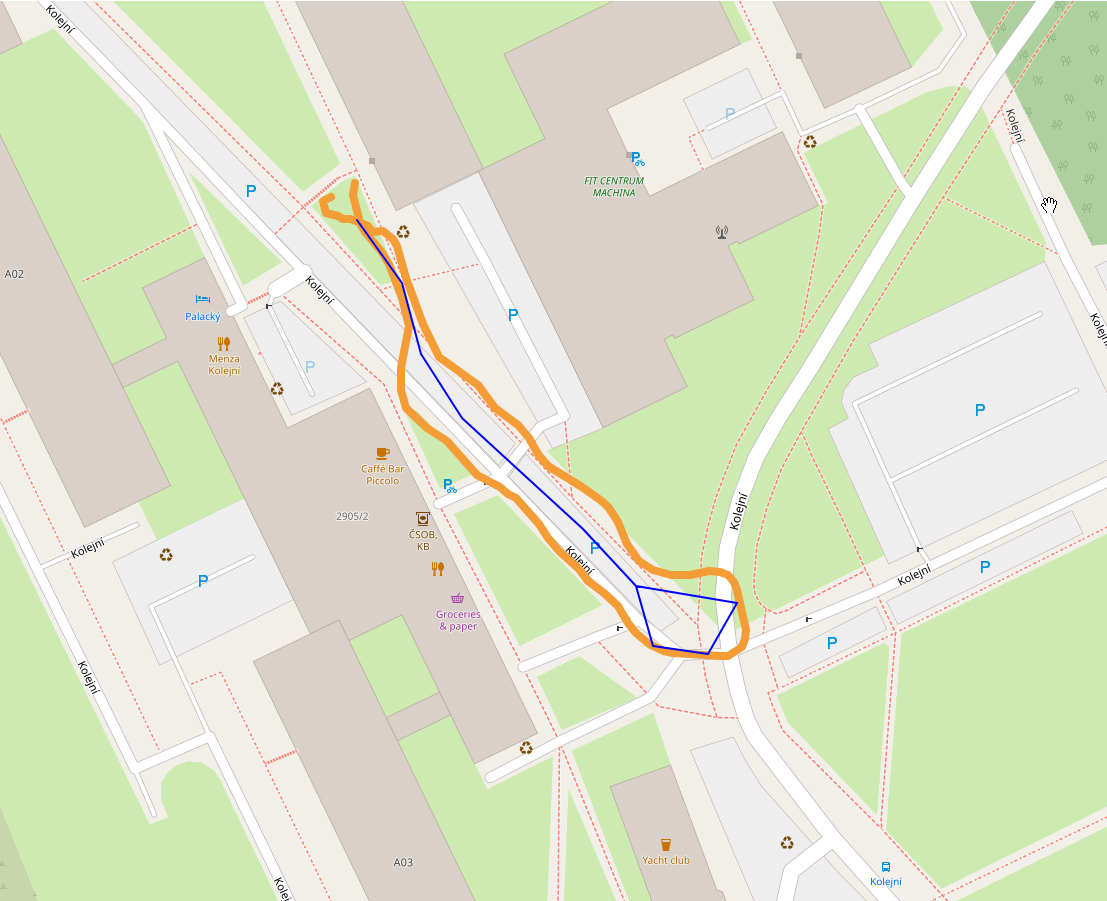
\includegraphics[width=0.85\textwidth]{obrazky/routeB.png}
  \caption{Filtrace cesty A}
  \label{filter_routeA}
\end{subfigure}
\vspace{1cm}
\begin{subfigure}
  \centering
  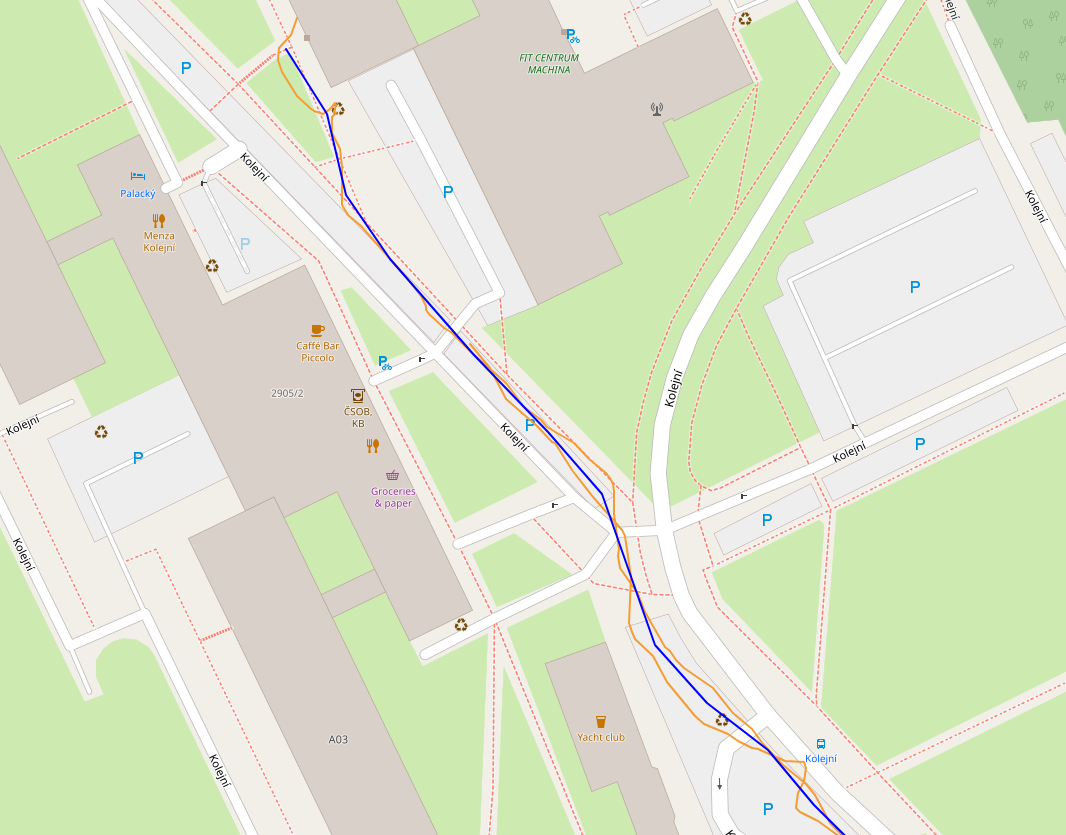
\includegraphics[width=0.85\textwidth]{obrazky/routeA.png}
  \caption{Filtrace cesty B}
  \label{filter_routeB}
\end{subfigure}
\end{figure}

\clearpage
\begin{figure}[h]
    \centering
    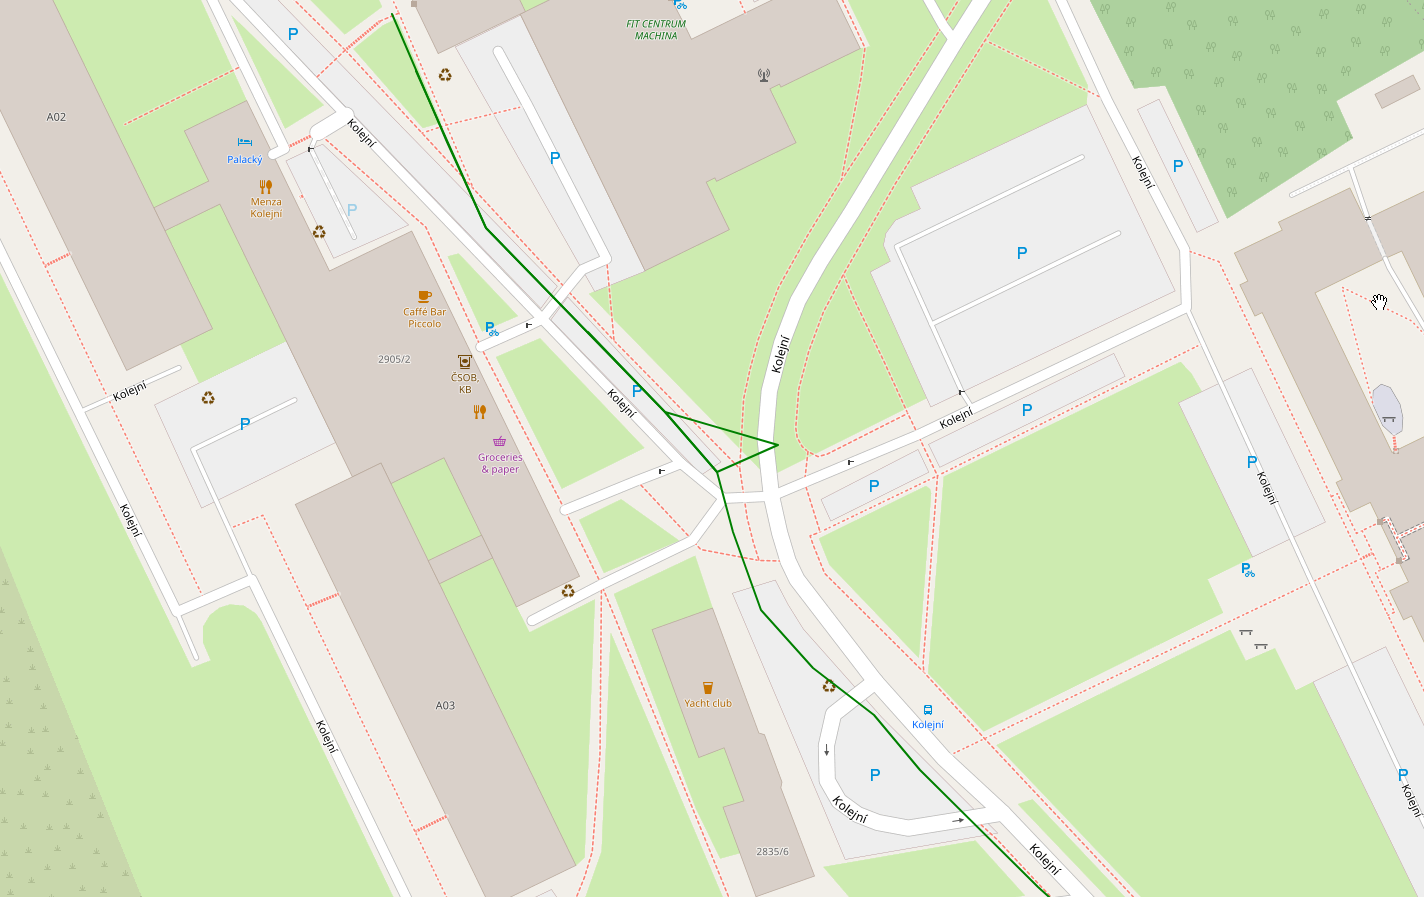
\includegraphics[width=0.85\textwidth]{obrazky/routeAB.png}
    \caption{Kombinace cesty A a~B}
    \label{filter_routeAB}
\end{figure}



\subsection{Přiřazení Voroného regionů}
Po dokončení filtrace uživatelské aktivity dochází k~přiřazení regionů k~aktivitě. Pro zlepšení výkonu API a je využita optimalizace v~C\#, která spočívá v~hromadném posílání požadavků. Cesta je rozdělena do skupin po 20 souřadnicích a~následně je pro každou vytvořen tzv. \emph{Task}. Následně se čeká na výsledek všech požadavků pomocí metody \emph{Task.WhenAll(tasks)}. Ty jsou na nižší programovací úrovni zpracovány paralelně pomocí vláken.~\cite{TaskThreads}

Úryvek kódu pro zpracování skupiny požadavků:
\begin{verbatim}
    var centeredRoute = new List<RouteCoordinate>();
    var numberOfBatches = (int)Math.Ceiling((double)route.Count / batchSize);
    for (var i = 0; i < numberOfBatches; i++)
    {
        var originalCoords = route.Skip(i * batchSize).Take(batchSize);
        var tasks = originalCoords.Select(x => 
        GetCenteredCoordinate(x.Latitude, x.Longitude);
        centeredRoute.AddRange(await Task.WhenAll(tasks));
    }
\end{verbatim}
V kódu lze vidět výpočet množství jednotlivých skupin dle nastavené velikosti\,--\,proměnná \texttt{numberOfBatches}. Následně je z pole vybráno požadované množství prvků a je vytvořené vlákno pro každou souřadnici. Po zpracování požadavků skrze \emph{Overpass API} je výstup přiřazený do pole \texttt{centeredRoute}.
\newpage
Pro každý požadavek je následně zavolaná metoda s~následujícím pseudokódem: 
\begin{verbatim}
    Na vstupu souřadnice zeměpisné šířky a délky: lat, lon
    Opakuj dokud není nalezen alespoň jeden střed regionu:
        Pošli požadavek:
            Nalezni středy regionů a okruh 10 metrů od lat,lon
        Pokud žádné neexistují: 
            Zvyš okruh o 20 metrů
    Pokud je více jak jeden střed:
        Najdi nejbližší střed k lat, lon
    Vrať souřadnice středu
\end{verbatim}
\emph{GET} Požadavek je vytvořen dle následující šablony:
\begin{verbatim}
    {URL}/api/interpreter?
         data=[out:json];
         node(around:{lookDistance},{lat},{lon});
         out geom;
\end{verbatim}
Proměnná lookDistance je okruh, ve kterém se hledají středy regionu. Lat a~lon jsou počáteční souřadnice z~uživatelovy trasy. Proměnná URL se může změnit dle konfigurace serveru, viz sekce~\ref{config}. 

Po zpracování celé cesty je cesta uložena jako samostatná, tvořená pouze ze středu regionů. Pokud se v~základní uživatelské cestě vyskytl více jak jeden bod uvnitř regionu, poté jsou i~ve výsledné cestě duplicitní hodnoty. Proto je před vytvořením dotazů je cesta zkontrolována a~duplicitní hodnoty jsou odstraněny. Toto podstatně ulehčí množství vyhledávání, které je nutné dělat v~databázi.

Pro získání hranic regionu je následně využita databáze popsaná v~sekci~\ref{SQLDB}. Pro každý střed regionu je vytvořen SQL dotaz. Toto je nejvíce procesorově náročná část z~důvodu množství regionů, a~tedy i~řádků v~databázi. Při testování byla průměrná doba zpracování jednoho dotazu kolem 500 milisekund. Relace s~výsledným regionem je uložena do pole a~zapsána do databáze. Je nutno vyhledávat dle desetinných čísel, tedy při vytvoření dotazu je potřeba zohlednit nepřesnost. Následující úryvek kódu popisuje zmíněný SQL dotaz: 
\begin{verbatim}
    var region = dbContext.StaticRegions.FirstOrDefault(x =>
        x.Index2 - 0.0000000001 <= coordinate.Latitude &&
        x.Index2 + 0.0000000001 >= coordinate.Latitude && 
        x.Index1 - 0.0000000001 <= coordinate.Longitude &&
        x.Index1 + 0.0000000001 >= coordinate.Longitude);
\end{verbatim}
Přesnost je nastavena na 10 desetinných míst a~odvíjí se od formátu zeměpisných souřadnic, které často dosahují většího množství desetinných míst. Přesnost samotná nemění náročnost vyhledávání dle testování. 
\section{Zobrazení dat}
Zobrazení dat je zprostředkované pomocí webové aplikace. Sekce probírá využité technologie a~některé implementační detaily. 

\subsection{Technologie webové aplikace}
Aplikace je implementovaná pomocí \emph{Vue}, dříve zmíněno v~sekci ~\ref{frameworks}, s~použitím \emph{Vuetify}. 
\subsubsection{Implementace rozhraní}
Pro implementaci rozhraní byl využit balíček nástrojů \emph{Vuetify}. Ten je postavený na základě dříve zmíněného \emph{Vue.js}. Cílem projektu je poskytnout vývojářům množství moderně vypadajících komponent, které se často na webu opakují. Následně je úkolem vývojáře je kreativně využít pro vytvoření unikátního webu. \emph{Vuetify} je vyvinuto na základě tzv. \emph{Material Design}, který specifikuje, aby každý komponent byl modulární, responzivní a~výkonný. V~nedávné minulosti bylo do světa vypuštěno \emph{Vue 3} a~díky aktivní komunitě je již dostupné i~\emph{Vuetify 3}, i~když stále v~beta verzi. Právě tato beta verze byla využita pro implementaci uživatelského rozhraní. \cite{vuetify}

\subsubsection{Změna zobrazení}
Pro konfiguraci přístupu uživatele je využitý nástroj \emph{Vue Router}. Zároveň se i~stará o~změnu zobrazení komponentů dle nastavené cesty v~prohlížeči. Manuálně je zde nastavena konfigurace za použití perzistentního úložiště. Když uživatel není přihlášen, tak ho router nenechá přistoupit na žádné jiné stránky, kromě přihlašovací. A~naopak, pokud je uživatel již přihlášen, tak není schopný se vrátit na přihlašovací obrazovku, aby nebyl vytvořený případný konflikt.
Útržek kódu z~nastavení \emph{Vue Router}:
\begin{verbatim}
        {
          path: "/auth",
          name: "auth",
          meta: {
            requiresGuest: true,
          },
          component: () => import("@/views/AuthView.vue"),
        }
\end{verbatim}
Následně router poskytuje metodu \emph{beforeEach}, která je zavolaná před každou změnou stránky. Zde je implementovaná konfigurace kontroly meta informací pro danou stránku v~porovnání s~přihlašovacím stavem uživatelského prohlížeče z~perzistentního úložiště. 
\subsubsection{Perzistentní uložení}
Při implementaci aplikace byla řešena otázka dočasného uložení malých uživatelských dat. Jedná se o~věci jako uživatelské jméno a~v~pozdějších fázi uložení přizpůsobení viditelnosti tras, uložení pozice a~přiblížení mapy.

Pro zajištění tohoto chování bylo implementované perzistentní úložiště pomocí nástroje \emph{Pinia}. V~minulosti \emph{framework Vue} využíval známý a~rozšířený nástroj \emph{Vuex}. Počátkem vývoje byl \emph{Pinia} experiment pro prozkoumání budoucích metod pro uložiště, co mohlo být \emph{Vuex 5}. Vývojáři ovšem zjistili, že \emph{Pinia} již implementuje větší množství základních konceptů, které by očekávali ve \emph{Vuex 5}, a~proto se \emph{Pinia} stala hlavním doporučeným nástrojem pro perzistentní uložení. \emph{Pinia} má jednodušší rozhraní a~obecně jednodušší přístup k~metodám, které poskytuje vývojáři. \cite{pinia}

V úložišti jsou například uchovány informace:
\begin{itemize}
    \item Stav přihlášení.
    \item Jméno uživatele.
    \item Pozice a~přiblížení mapy.
    \item Přiřazené barvy k~aktivitě a~k regionu.
\end{itemize}
V~úložišti se také vyskytují proměnné, které si klient ukládá pro jednodušší komunikaci mezi jednotlivými prvky stránky. Například, chybové hlášení při selhání požadavku na API je reaktivně nastaveno na proměnnou, která je uložena v~hlavním úložišti. Nejvíce uživatel ocení perzistentní uložení, když prochází mezi jednotlivými režimy zobrazení a~aplikace udržuje stav, který si uživatel nastavil v~předchozích krocích.

\subsection{Komponent mapy}
Jako komponent pro zobrazení dat byl vybrán nástroj na bázi \emph{OpenLayers}. Hlavním důvodem byla jednoduchá integrace s~\emph{Vue frameworkem} pomocí podpurné knihovny \emph{vue3-openlayers}\footnote{Github knihovny: \url{https://github.com/MelihAltintas/vue3-openlayers}}. Ta poskytuje komponent mapy kompatibilní s~reaktivními vlastnostmi \emph{vue3}. Mapa následně může zobrazovat data na množství rastrových a~vektorových vrstvách. \cite{openlayers1}
\subsection{Komunikace s~API}
\label{httpreq}
Komunikace s~API je zajištěna pomocí HTTP požadavků. Na nízké úrovni je syntaxe každého požadavku tvořena z~definice typu metody požadavku, hlaviček HTTP a~následně dat. Nejvíce používané metody požadavku jsou tzv. \emph{GET, PUT, POST, DELETE} metody. Dále existují i~metody \emph{HEAD, TRACE, CONNECT}, ty ovšem nebyly pro implementaci komunikace využity. \emph{GET} metoda je nejspíše nejpopulárnější metoda ze všech, je to typ metody, který prohlížeč využívá pro stáhnutí obsahu webové stránky po kliknutí na jakékoliv URL. Metoda \emph{GET} se také používá v~HTML formulářích, kdy při definice formuláře je možné specifikovat použitou metodu. Zde se ovšem vyskytuje bezpečnostní riziko. V~požadavku typu \emph{GET} se obecně nevyužívá tělo pro předání dat, ale parametry adresy jako tzv. \emph{query}. V~aplikaci je \emph{GET} metoda použita hlavně na požadavky již zpracovaných dat, tedy pro získání dat uživatele. Implementaci metody \emph{POST} v~minulosti lze považovat za jeden z~největších pokroků webové komunikace. Umožňuje webovým stránkám být doopravdy interaktivní. V~aplikaci je využita pro sdělení serveru, aby provedl určitou akci. Jmenovitě dává API sdělení, že si uživatel přeje např. načíst nové aktivity ze Stravy, přihlásit a~odhlásit se. \emph{PUT} není tak obvyklá metoda jako \emph{GET} nebo \emph{POST}, využívá se nejčastěji k~poslání serveru větší množství dat. V~rámci aplikace nebylo nutné ji nikde využít. \emph{DELETE} má opačné využití oproti \emph{PUT}, je využit pro sdělení serveru pro odstranění určitého obsahu. V~rámci aplikace se zde jedná hlavně o~smazání jednotlivých aktivit nebo smazání svého uživatelského účtu.~\cite{httprequests}

Pro zprostředkování požadavků byla v~aplikaci využita knihovna \emph{Axios}. Je to JavaScriptová knihovna s~podporou prohlížečů a~\emph{Node} (základní \emph{framwork} pro \emph{Vue, Vuetify}), využívá i~koncept \emph{slibů} (angl. \emph{Promises}). \emph{Promises} nám v~aplikaci umožňují asynchronní zpracování požadavků, dá se říci, že určité data jsou \uv{slíbeny} a~následně aplikace může počkat na odpověď API i~při využití asynchronních požadavků pomocí známých příkazů \emph{await}  a~\emph{async}. V~aplikaci \emph{Axios} usnadňuje posílání jednotlivých požadavků díky globální konfiguraci. Zde se dají jednoduše nastavit nutné parametry, jako je URL API, typ obsahu a~umožnění komunikace mezi webovými doménami -- CORS, dále rozebrané v~sekci~\ref{apiimplementation}.~\cite{axios}


Následuje útržek kódu konfigurace \emph{Axios}, je v~něm vidět nastavení adresy serverového API, kde se zpracovávají požadavky aplikace. Je nutné také přikládat hlavičky a~povolit CORS pomocí \emph{crossDomain} atributu. 
\begin{verbatim}
        const config = {
            baseURL: "http://localhost:7040/",
            headers: {
            "Content-type": "application/json",
            },
            withCredentials: true,
            crossDomain: true,
        };
\end{verbatim}
Dále je volání jednotlivých požadavků implementováno v~souboru \emph{UserService.ts}, což je třída zapsaná pomocí \emph{TypeScript}.

\subsubsection{Zpracování odpovědí}
V API jsou data po komunikaci s~databázi uložena do C\# tříd. Následně v~reakci na požadavek na daný koncový bod je \emph{Entity Framework} serializuje do podoby JSON (angl. \textit{JavaScript Object Notation}) a~jsou odeslány jako odpověď. Pro jednoduché zpracování na straně klienta jsou obdobným způsobem vytvořeny třídy v~\emph{TypeScript}. \emph{TypeScript} je nadstavba \emph{JavaScriptu}, přibližuje svět programování viditelnou část webové stránky blíže k~programování \emph{.NET} pomocí objektově orientovaného programování. Za cíl si uložil tvorbu svého vlastního standardu pro tvorbu moderních webových aplikací, k~dosažení tohoto cíle pomáhá fakt, že \emph{Typescript} je otevřený software, s~otevřeným zdrojovým kódem a~jeho vývojáři naslouchají uživatelům při dalším vývoji. \cite{typescript}

Následující útržek kódu ze souboru \emph{activity.ts} třídy Activity popisuje základní informace o~aktivitě, které \emph{frontend} očekává v~reakci na požadavek:
\begin{verbatim}
    export default class Activity {
        public name: string;
        public id: number;
        public elapsedTime: number;
        public startDate: string;
        
        constructor(name: string, id: number,
        elapsedTime: number, startDate: string) {
            this.name = name;
            this.id = id;
            this.elapsedTime = elapsedTime;
            this.startDate = new Date(startDate).toLocaleDateString();
        }
    }
\end{verbatim}
\newpage
\section{Funkce webu pro uživatele}
\label{appfunctions}
Pro uživatelský komfort bylo implementováno několik funkcí. Jedná se například o~komponentu zobrazující načítání zpracování aktivit. Když uživatel přistoupí na stránky, kde se obvykle zobrazují Voroného regiony nebo zprůměrované aktivity, ale server stále nedokončil zpracování těchto aktivit, uživateli se zobrazí komponent kolečka s~číselným zobrazením současného stavu načtení v~\%. Toto je implementované pomocí opakovaných požadavků ze strany klienta na API, následně server jako odpověď vrátí stav zpracování, který je uložen do proměnné. Ta je reaktivně propojena s~komponentem načítání. Přestože není dokončeno zpracování, tak si uživatel může zobrazit jednotlivé aktivity v~základní podobě načtené ze Stravy. Pokud má uživatel nahráno větší množství aktivit, je zobrazen komponent stránkování. Zde si uživatel může zvolit, kolik aktivit chce vidět na jedné stránce a~procházet jednotlivými stránkami. Po kliknutí na aktivitu se aktivita rozevře a~uživatelovi se klientské zobrazení automaticky upraví tak, aby mapa aktivity byla celá viditelná na jeho obrazovce. Dále jsou zde k~přečtení zajímavé detaily o~aktivitě, které jsou dostupné ze Stravy. Po dokončení zpracování aktivit se uživateli umožní možnost smazat jednotlivé aktivity. Tyto tlačítka jsou vypnuté během zpracování z~důvodu práce v~pozadí na serveru a~následně složitému zastavování práce, která již probíhá v~\emph{Hangfire}. 

Při zobrazení regionů nebo filtrovaných tras si uživatel dále může upravit zobrazení dle své libosti. Při prvním načtení stránky jsou k~jednotlivým trasám přiřazeny náhodně barvy ze seznamu barev. Ty si uživatel může změnit v~menu, které se zobrazuje na pravé straně obrazovky. Zde jsou na výběr možnosti jako změna barvy regionu nebo jednotlivých tras a~tloušťka hranice regionů. Popřípadě se v~tomto nastavení lze i~nastavit hranice jako průhledné.

Uživatel může smazat jednotlivé aktivity z~databáze aplikace. Již při zpracování si server ukládá informace o~tom, které aktivity se navzájem ovlivňují. Například, pokud se dvě aktivity navzájem filtrovaly, tak si server ukládá tuto informaci. Po smazání dojde k~chytrému přepočítání aktivit, zároveň se uživateli znovu zobrazí komponent pro stav načítání, která se aktualizuje. Pokud si uživatel přeje vrátit některé ze smazaných aktivit, tak si může \uv{Resetovat účet} po kliknutí na svoje jméno v~pravém horním rohu obrazovky. 
Aplikace aktualizuje a~stahuje nové aktivity po každém přihlášení. Ovšem uživatel se nepřihlašuje příliš často díky nastavení aplikace na pamatování uživatele, takže bylo přidáno tlačítko pro manuální spuštění aktualizace aktivit. Během dalšího vývoje je možné využít tzv. \emph{Webhooks}, které poskytuje Strava. Ve své podstatě jsou to požadavky, které pošle Strava na registrované API, pokud jeden z~jeho autorizovaných uživatelů nahraje novou aktivitu\footnote{Strava API Webhooks dostupné z: \url{https://developers.strava.com/docs/webhooks/}}. Toto nebylo implementované z~důvodu využití lokálních serverů po drtivou většinu vyvíjeného času, \emph{Webhooks} fungují pouze na veřejně dostupném API.

Aplikace byla vytvořena pomocí moderních technologií, které umožnily lehkou implementaci responzivního chování. Pokud uživatel přistoupí na webovou aplikaci pomocí klienta s~omezenou šířkou prohlížeče, tak se aplikace přizpůsobí. Tyto změny jsou hlavně přesunutí hlavního navigačního menu do tzv. \emph{hamburgeru} ve formě tří horizontálních úseček signalizující rozevírací seznam. Po kliknutí na tuto ikonku se znovu objeví celý navigační seznam. Podobné chování se zároveň děje na pravé straně obrazovky, kdy se menu pro přizpůsobení zobrazení aktivit a~regionů schová. Místo menu se objeví šipka, která po kliknutí seznam znovu zobrazí uživateli. 

\chapter{Testování}
Kapitola ukazuje výsledky implementace a~její následné testování proti uživatelské chybě.
\section{Přihlášení uživatele}
Při řešení přihlášení bylo hlavně testované případné zamítnutí autorizace. Pokud klient nezíská správné povolení, uživateli se zobrazí chybová hláška vysvětlující problém. Toto chování lze vidět v~obrázcích~\ref{test:login_cancel} a~\ref{test:login_fail}.

\section{Seznam aktivit} 
Obrázek~\ref{test:activity_list} zobrazuje webovou stránku po úspěšném přihlášení uživatele. Je zde vidět seznam aktivit i~stránkování. Součásti testu bylo měnění komponentu stránkování, například vložení textu na špatné místo, což by aplikaci mohlo rozbít\,--\,dle výsledku testu nelze pomocí stránkování zobrazený seznam rozbít. Po plném načtení aktivit se tlačítka pro smazání sama zpřístupnila, dle dokumentace v~sekci~\ref{appfunctions}. Obrázek~\ref{test:activity_detail} zobrazuje výsledek kliknutí na aktivitu, kdy se otevřel její detail obsahující i~trasu běhu. Zde jsou také vidět, že po najetí kursorem se uživateli zobrazí dodatečné akce účtu jako jeho resetování nebo smazání.

\section{Mazání aktivit}
Po smazání aktivit, které se neovlivňují, nedošlo k~žádnému přepočítávání a~aplikace ihned zpřístupnila plnou funkcionalitu. Před úplným smazáním jakéhokoliv prvku se uživateli vždy zobrazí potvrzovací dialog, který dynamicky mění obsah dle mazaného objektu, a~tedy zmenšuje šanci náhodné a~nechtěné uživatelovi akce. Dialog je viditelný v~obrázku~\ref{test:dialog}.

Po smazání všech aktivit z~účtu aplikace správně zobrazila stránku, která uživatele informuje o~neexistenci žádných aktivit dle obrázku~\ref{test:app_empty}. Reakce na jednotlivé akce jsou v~některých případech opožděné, to se děje hlavně z~důvodu vzdálenosti databáze a~lokálního API. Během doby zpracování aktivit se uživateli korektně zobrazoval komponent pro načítání, jak lze vidět v~obrázku~\ref{test:loading}. 

Obdobně bylo testováno i~mazání a~resetování účtu na stránkách zobrazující zabrané území a~filtrované cesty.

\section{Voroného mapa a~filtrované cesty}
Stránky zobrazující vypočítané zabrané území uživatele a~filtrované trasy fungují responzivně a~zobrazují data. Voroného regiony nejsou naprosto přesné, v~malém procentu případu se stává, že uživatel projde region, ale není mu přiřazen. V~rámci testování jediný možný důvod, který může stát za nepřesností, je výpočet samotných regionů dle knihovny \emph{Scipy}. Toto chování může nastat obzvláště, pokud uživatel projde blízko hranice samotného regionu. Ukázka responzivní aplikace je na obrázku~\ref{test:responsive}. 

V předešlých sekcích (obrázek~\ref{filter_routeAB}) byla trasa zobrazena pomocí \emph{Leaflet}. Nyní lze na obrázku~\ref{test:filterAB} ve webové aplikaci vidět stejnou trasu, zobrazenou pomocí \emph{OpenLayers}.

\chapter{Závěr}
Na závěr jde říci, že všechny body bakalářské práce byly splněny. Cílem bylo vytvořit webovou aplikaci zobrazující území rozdělené dle Voroného regionů, které se přiřazují dle trasy. 

V kapitole \ref{theory} byl vykonaný průzkum problematiky \emph{OpenStreetMap, GPS} a~dostupných fitness aplikací. Na základě průzkumu bylo pro záznam dat rozhodnuto využití již existující mobilní aplikace. Vývoj nové mobilní aplikace by v~rámci bakalářské práce byl možný, ale nikdy by se kvalitou zpracování nevyrovnal již existujícím konkurentům. Toto propojení navíc umožňuje uživateli využít jeho dříve zaznamenané aktivity. Jako hlavní zdroj dat byla vybraná aplikace Strava, která má nejlepší podporu vývojářů třetí strany. 

V následující kapitole byly shrnuty uživatelské případy užití, pro jednoduchost a~přehlednost zobrazeny ve formě modelu. Na základě průzkumu popsaném v~sekci~\ref{frameworks} byla pro implementaci serverové a~klientské části zvolena technologie \emph{Vue} a~\emph{ASP .NET}. Po porovnání různých typů vyšla najevo jasná výhoda při využití relační databáze. Dle popisu v~sekci~\ref{olvsleaflet} nebylo zřejmé, která technologie se více hodí pro implementaci uživatelského zobrazení. Pro názorné zobrazení návrhu uživatelského rozhraní byly vytvořeny tzv. \emph{Wireframe}, viz sekce~\ref{wireframes}.

Kapitola čtvrtá se dá považovat za nejdůležitější kapitolu. Obsahuje popsané základy celé implementace, včetně využitých technologií. Na počátku je vysvětlené, jakými způsoby jsou vypočteny data jednotlivých Voroného regionů a~jak jsou vloženy do databáze. Pro tvorbu samotné databáze byla zvolen \emph{Code-First} přístup, který poskytuje \emph{Entity Framework v~C\#}. Následně jsou zde řešeny otázky přihlášení, autentizace a~zpracování dat. Pro filtraci cest byl implementovaný vlastní algoritmus na základě vzdálenosti jednotlivých souřadnic aktivit. Pro přiřazení zabraného území uživateli byla využita kombinace API od vývojářů OpenStreetMap\,--\,Overpass adatabáze. Pro zobrazení těchto vypočítaných dat byla pomocí technologií \emph{Vue a~Vuetify} vytvořena webová aplikace. V~kapitole byla také řešena otázka responzivity z~důvodu velkého množství uživatelů mobilních telefonů. 

Z testování vyplynulo, že v~určitých částech rychlost zpracování aktivit může být snížena z~důvodu hardwarových omezení. Také je zde malá šance, že region nebude přiřazen kvůli problému přesnosti.
\label{webapp}
